\documentclass{prgrado}

\usepackage[
    backend=biber,
    style=alphabetic,
    maxbibnames=99,
]{biblatex}

% Hace que el + de las citas cuando hay demasiados autores sea un superscript
\renewcommand*{\labelalphaothers}{\textsuperscript{+}}

% Agranda las filas de las tablas
\renewcommand{\arraystretch}{1.5}

% Interlineado
\renewcommand{\baselinestretch}{1.2}

% Traté de que dijera "Tabla" en las captions de las tablas en lugar de "Cuadro"
% No funcionó :(
% \usepackage{babel}[spanish]
% \usepackage{caption}
% \renewcommand{\tablename}{Tabla}

\usepackage{subcaption}
\usepackage{amsfonts}
\usepackage{amsmath}

\addbibresource{referencias.bib}

% título del proyecto (debe escribirse en minúscula, con excepción de la
% letra inicial de la primera palabra y nombres propios)
\title{Fingxels}

% autores
\author{Francisco Aguirre, Felipe Pizzorno}

% fecha de la defensa
\date{\today} % TODO: Change

% supervisor
\supervisor{Eduardo Fernández}

% cosupervisor (comentar si no tiene)
% \cosupervisor{Jose Pedro Aguerre}

% licencia creative commons del documento
% opciones: by, by-sa, by-nd, by-nc, by-nc-sa y by-nc-nd
% opción por defecto: by-nc-nd versión 4.0
\cclicense{by}{4.0}

%%%%%%%%%%%%%%%%%%%%%%%%%%%%%%%%%%%%%%%%%%%%%%%%%%%%%%%%%%%%%%%%%%%%%%%%%%%%%%%%%%%%%%%%%%%%%%%%

%links con colores 
\hypersetup{
  colorlinks   = true,
  urlcolor     = blue,
  linkcolor    = blue,
  citecolor    = blue
}

\graphicspath{{figures/}}

\begin{document}

%%%%%%%%%%%%%%%%%%%%%%%%%%%%%%%%%%%%%%%%%%%%%%%%%%%%%%%%%%%%%%%%%%%%%%%%%%%%%%%%%%%%%%%%%%%%%%%%
% Parte inicial
%%%%%%%%%%%%%%%%%%%%%%%%%%%%%%%%%%%%%%%%%%%%%%%%%%%%%%%%%%%%%%%%%%%%%%%%%%%%%%%%%%%%%%%%%%%%%%%%

\frontmatter % numeración en romanos, capitulos sin numerar

% carátula
\maketitle

%%%%%%%%%%%%%%%%%%%%%%%%%%%%%%%%%%%%%%%%%%%%%%%%%%%%%%%%%%%%%%%%%%%%%%%%%%%%%%%%%%%%%%%%%%%%%%%%

% agradecimientos
\chapter*{Agradecimientos}

Agradecer, siempre es bueno agradecer. % TODO: Hacer a lo último

%%%%%%%%%%%%%%%%%%%%%%%%%%%%%%%%%%%%%%%%%%%%%%%%%%%%%%%%%%%%%%%%%%%%%%%%%%%%%%%%%%%%%%%%%%%%%%%%

% resumen
\chapter*{Resumen}

% El resumen (200-500 palabras) debe dar una idea completa de todo el
% proyecto, mencionando claramente los formalismos, técnicas, herramientas y lenguajes
% utilizados. No debe limitarse a describir el problema abordado, sino que debe describir
% la solución del problema, con una evaluación de la misma. No debe incluir referencias
% bibliográficas ni referencias a otras partes del informe. Tampoco debe utilizar
% acrónimos sin explicar su significado.

En este trabajo se aborda el problema de la iluminación global en tiempo real, un problema desafiante y relevante en la industria de los videojuegos, cine, simulaciones y la computación gráfica en general.
La mayoría de las técnicas de iluminación global se basan en el método de Monte Carlo, y esto las hace computacionalmente costosas, requiriendo hardware especializado y técnicas de aprendizaje automático para alcanzar el tiempo real.

En este contexto, se hace foco en el algoritmo de \textit{voxel cone tracing}, una técnica de trazado de conos que usa una estructura de datos basada en vóxeles que se ha demostrado prometedora por su capacidad para producir efectos de iluminación global de alta calidad en tiempo real sin necesidad de hardware especializado.

El objetivo principal de este trabajo es crear una implementación open source del algoritmo de \textit{voxel cone tracing} y probarla en hardware moderno. La implementación realizada no solo demuestra la viabilidad y eficacia de la técnica en un entorno de hardware actual, sino que también es un recurso didáctico valioso para cualquier persona interesada en aprender acerca de computación gráfica, iluminación global y su implementación.

Para esta implementación, se utilizaron principalmente las herramientas Rust y OpenGL, debido a su alto rendimiento, abundancia de documentación y simplicidad.
El algoritmo corre exclusivamente en la GPU, aprovechando la alta paralelización que esta provee.
Su desarrollo se realizó en Linux, pero el programa no está limitado a este sistema operativo dado que puede ser portado fácilmente a otros.

Para evaluar la implementación, se realizaron experimentos en hardware moderno y se compararon los resultados con implementaciones previas de la técnica.

El código del motor se encuentra en el siguiente repositorio:

\url{https://github.com/franciscoaguirre/voxel-cone-tracing}

\hfill \break
\keywords{Voxel cone tracing, Iluminación global, OpenGL, Rust}

%%%%%%%%%%%%%%%%%%%%%%%%%%%%%%%%%%%%%%%%%%%%%%%%%%%%%%%%%%%%%%%%%%%%%%%%%%%%%%%%%%%%%%%%%%%%%%%%

% índice
\tableofcontents
\newpage


%%%%%%%%%%%%%%%%%%%%%%%%%%%%%%%%%%%%%%%%%%%%%%%%%%%%%%%%%%%%%%%%%%%%%%%%%%%%%%%%%%%%%%%%%%%%%%%%
% Parte central
%%%%%%%%%%%%%%%%%%%%%%%%%%%%%%%%%%%%%%%%%%%%%%%%%%%%%%%%%%%%%%%%%%%%%%%%%%%%%%%%%%%%%%%%%%%%%%%%

\mainmatter %numeración en arábicos, numerar capítulos 

% introducción
\graphicspath{{chapters/5_experimentos/figures/}}

\chapter{Experimentación}\label{chap:experiments}

Para analizar el rendimiento de la implementación, se realizaron experimentos en distintas tarjetas gráficas, las cuales se ven en el Cuadro \ref{tab:hardware-used}.
Estas, $H1$, $H2$ y $H3$, corresponden a hardware con capacidades gráficas progresivamente superiores.
Las escenas utilizadas se muestran en las figuras \ref{fig:cornell-box-full} y \ref{fig:sponza}, que llamaremos $S1$ y $S2$ respectivamente.
Se puede observar en cada una de ellas la luz indirecta difusa, luz indirecta especular y sombras suaves.

\begin{table}[ht]
	\centering
	\begin{tabular}{|c|c|c|c|c|}
		\hline
		\textbf{Nombre} & \textbf{GPU} & \textbf{Núcleos} & \textbf{Clock (GHz)} & \textbf{VRAM (GB)} \\
		\hline
		$H1$ & Intel Mesa ADL GT2 & 96 & 1.45 & * \\
		\hline
		$H2$ & Nvidia GTX 1660 Ti mobile & 1536 & 1.45 & 6 \\
		\hline
		$H3$ & Nvidia Geforce RTX 4070 & 5888 & 1.92 & 12 \\
		\hline
	\end{tabular}
	\caption{Hardware utilizado. * al ser una tarjeta integrada, no tiene memoria gráfica dedicada.}
	\label{tab:hardware-used}
\end{table}

\begin{figure}[H]
	\centering
	  \begin{subfigure}{0.49\textwidth}
	      \centering
	  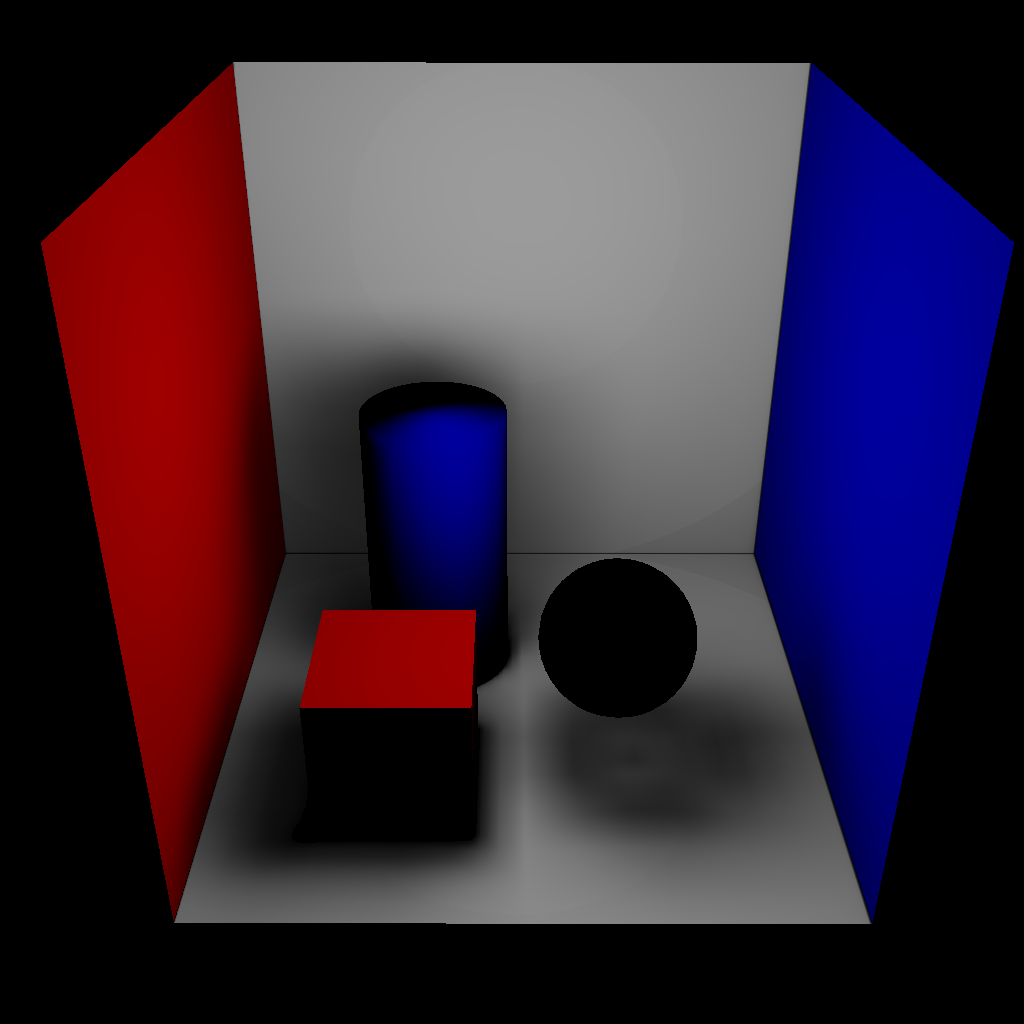
\includegraphics[width=\textwidth]{cornell-box-direct.png}
	      \caption{Solo luz directa.}
	  \end{subfigure}
	  \begin{subfigure}{0.49\textwidth}
	      \centering
	  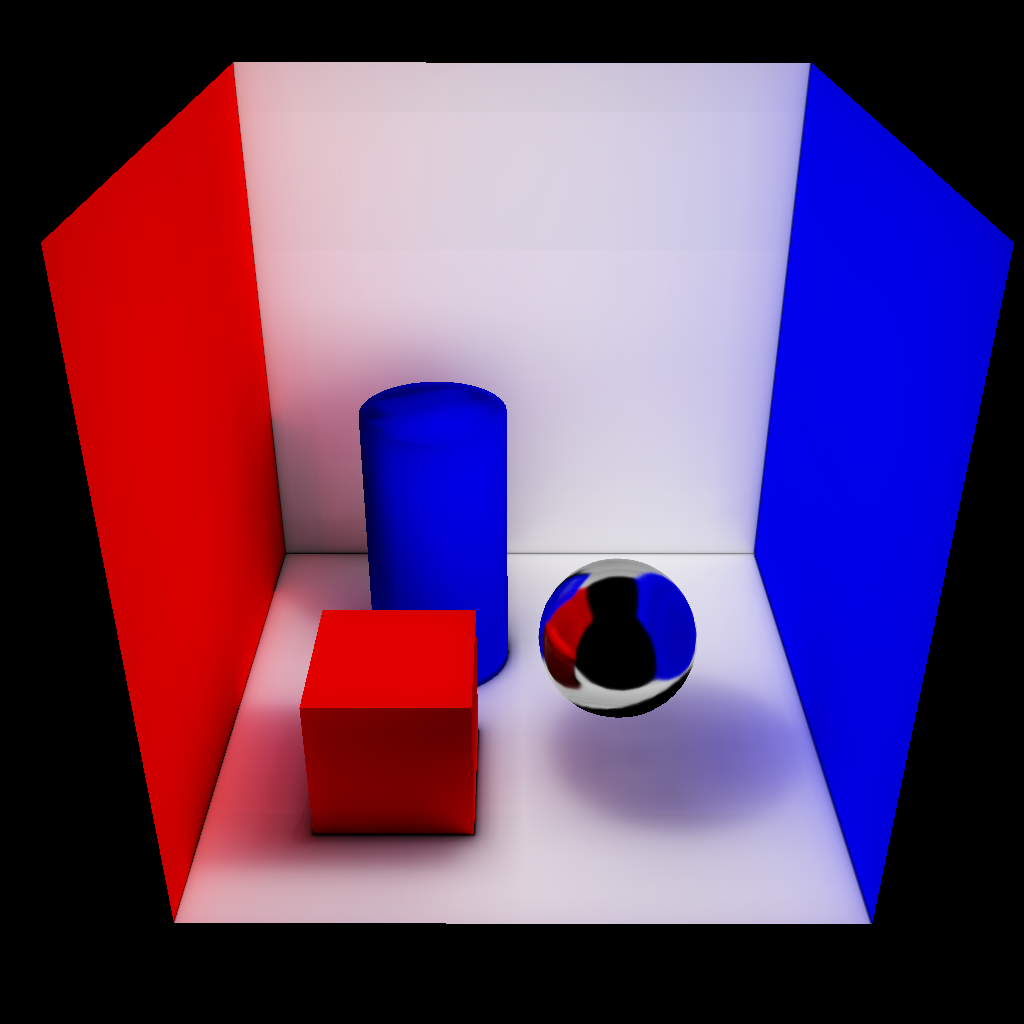
\includegraphics[width=\textwidth]{cornell-box-full.png}
	      \caption{Luz directa e indirecta.}
	  \end{subfigure}
	\caption{Escena de prueba con geometría simple.}
	\label{fig:cornell-box-full}
\end{figure}

\begin{figure}[H]
	\begin{subfigure}{0.49\textwidth}
	  \centering
	  \includegraphics[width=\textwidth]{sponza-direct.png}
	  \caption{Solo luz directa.}
	\end{subfigure}
	\begin{subfigure}{0.49\textwidth}
	  \centering
	  \includegraphics[width=\textwidth]{sponza-all.png}
	  \caption{Luz directa e indirecta.}
	\end{subfigure}
	\caption{Sponza.}
	\label{fig:sponza}
\end{figure}

Los experimentos varían la cantidad de vóxeles por dimensión, y registran los cuadros por segundo alcanzados (FPS, por sus siglas en inglés) y el tiempo de construcción del \textit{octree} en segundos.
Para conseguir los FPS se ejecutó el programa durante un minuto, tomando una muestra cada segundo, luego se promediaron.
Para el tiempo de construcción del \textit{octree}, se construyó 50 veces y se calculó el tiempo promedio.
Cada ejecución se realizó independientemente, para evitar posibles mejoras debido al uso del caché.

En el Cuadro \ref{tab:experiment-results} se muestran los resultados de estos experimentos en los 3 hardwares utilizados ($H1$, $H2$ y $H3$) descritos en el Cuadro \ref{tab:hardware-used}.
Se muestran los resultados para cada una de las escenas $S1$ y $S2$, en cada uno de los hardwares, y para cada nivel de resolución (vóxeles por dimensión).

\begin{table}[ht]
\centering
\begin{tabular}{|c|c|c|c|c|}
	\hline
	\textbf{Escena} & \textbf{Hardware} & \textbf{Vóxeles} & \textbf{FPS} & \textbf{Construcción del \textit{octree} (s)} \\
	\hline
	$S1$ & $H1$ & $256$ & $18.22$ & $1.76$ \\
	\cline{3-5}
	 & & $512$ & $14.77$ & $1.82$ \\
	\cline{3-5}
	 & & $1024$ & $12.13$ & $2.01$ \\
	\cline{2-5}
	 & $H2$ & $256$ & $136.57$ & $1.78$ \\
	\cline{3-5}
	 & & $512$ & $108.67$ & $1.80$ \\
	\cline{3-5}
	 & & $1024$ & $60.24$ & $1.89$ \\
	\cline{2-5}
	 & $H3$ & $256$ & $141.57$ & $1.88$ \\
	\cline{3-5}
	 & & $512$ & $141.47$ & $1.90$ \\
	\cline{3-5}
	 & & $1024$ & $140.88$ & $1.89$ \\
	\hline
	$S2$ & $H1$ & $256$ & $7.30$ & $1.84$ \\
	\cline{3-5}
	 & & $512$ & $4.29$ & $1.86$ \\
	\cline{3-5}
	 & & $1024$ & $2.84$ & $2.07$ \\
	\cline{2-5}
	 & $H2$ & $256$ & $59.68$ & $1.82$ \\
	\cline{3-5}
	 & & $512$ & $37.42$ & $1.94$ \\
	\cline{3-5}
	 & & $1024$ & $9.83$ & $1.83$ \\
	\cline{2-5}
	 & $H3$ & $256$ & $141.27$ & $1.70$ \\
	\cline{3-5}
	 & & $512$ & $141.51$ & $1.91$ \\
	\cline{3-5}
	 & & $1024$ & $141.21$ & $1.99$ \\
	\hline
\end{tabular}
\caption{FPS y tiempo de construcción del octree para cada escena.}
\label{tab:experiment-results}
\end{table}

\section{Análisis de resultados}

Una primera observación es que los cuadros por segundo se encuentran cerca del tiempo real.
Se nota que en $H1$ los FPS nunca superan los 20, mientras que en $H3$ nunca bajan de 140.
$H2$ representa un término medio, logrando más de 60 FPS en la escena simple ($S1$) y mostrando una gran variedad de valores en la escena compleja ($S2$) para cada resolución utilizada ($256$, $512$, $1024$).

Se observa que, como es de esperarse, a mayor resolución (vóxeles por dimensión), los cuadros por segundo disminuyen.
Esto se debe a que una resolución más alta mejora la aproximación y genera imágenes de mayor calidad, pero a costa de mayor carga computacional.

Un aspecto que destaca especialmente es el tiempo de construcción del octree, que permanece alrededor de los 2 segundos, cuando idealmente debería estar en el rango de los milisegundos.
Dado que este tiempo es prácticamente igual tanto en $H1$ como en $H3$, parece evidente que el cuello de botella no es la GPU en sí, sino la comunicación entre GPU y CPU.


% antecedentes
\graphicspath{{chapters/2_antecedentes/figures/}}

\chapter{Revisión de antecedentes}

% Idea:
% 1. ¿Qué es la luz?
% 2. Unidades de luz
% 3. Iluminación local y global
% 4. BRDF
% 5. Trazado de rayos
% 6. Trazado de conos
% 7. Photon Mapping
% 8. Vóxeles (acá van a haber integrales, rendering científico)
% 9. Octrees
% 10. Ducto gráfico
% 11. Rendering diferido
% ... no se si esto va acá ...
% 12. Teoría de pre-filtrado
% 13. Ray marching

En este capítulo se explicaran en detalle los conceptos teóricos y los antecedentes más importantes para entender el algoritmo de \textit{voxel cone tracing} y la implementación desarrollada.

\section{¿Qué es la luz?}

Antes de definir el problema de la iluminación global en computación gráfica y hablar de diversos trabajos que se han realizado al respecto, conviene dar un paso atrás y preguntarnos, ¿qué es la luz?
Esta pregunta es relevante porque, más allá de las variaciones, la gran mayoría de técnicas de iluminación global se basan en modelar a la luz físicamente.

El libro \textit{Physically Based Rendering}, de Pharr, Jakob y Humphreys \cite{pbr} brinda una explicación clara y resumida de la historia de la interacción entre los humanos y la luz.
La percepción a partir de la luz es central para nuestra existencia.
La incógnita de la naturaleza de la luz ha ocupado las mentes de grandes filósofos y físicos desde el comienzo de los tiempos.
La antigua escuela filosófica hinduista de Vaisheshika (siglos 5 a 6 antes de cristo) veía a la luz como una colección de pequeñas partículas viajando a través de rayos a una alta velocidad.
En el siglo 5 antes de cristo, el filósofo griego Empédocles postulaba que un fuego divino emergía de los ojos humanos y combinado con los rayos de luz del sol producía visión.
Entre los siglos 18 y 19, eruditos como Isaac Newton, Thomas Young, Augustin-Jean Fresnel desarrollaron teorías conflictivas, donde algunas modelaban la luz como consecuencia de la propagación de ondas, y otras de partículas.
Al mismo tiempo, André-Marie Ampère, Joseph-Louis Lagrange, Carl Friedrich Gauß, y Michael Faraday investigaban las relaciones entre electricidad y magnetismo que culminaron en la repentina y dramática unificación de James Clerk Maxwell en una teoría combinada conocida como \textbf{electromagnetismo}, \cite{maxwell-equations}.

La luz es una manifestación con propiedades de onda.
El movimiento de partículas eléctricamente cargadas, como electrones dentro del filamento de una bombilla, produce un disturbio en un campo eléctrico circundante que se propaga hacia fuera de la fuente.
La oscilación eléctrica también produce una oscilación secundaria de un campo magnético, que a su vez refuerza la oscilación del campo eléctrico, y así sucesivamente.
La interacción entre estos dos campos da lugar a una onda que se autopropaga y puede viajar distancias extremadamente largas.
Una representación de esto se puede ver en la figura \ref{fig:electromagnetic-wave}, en la que el campo eléctrico (azul) y el magnético (rojo) son perpendiculares el uno al otro y se propagan, avanzando a lo largo de un eje central.

\begin{figure}
    \centering
    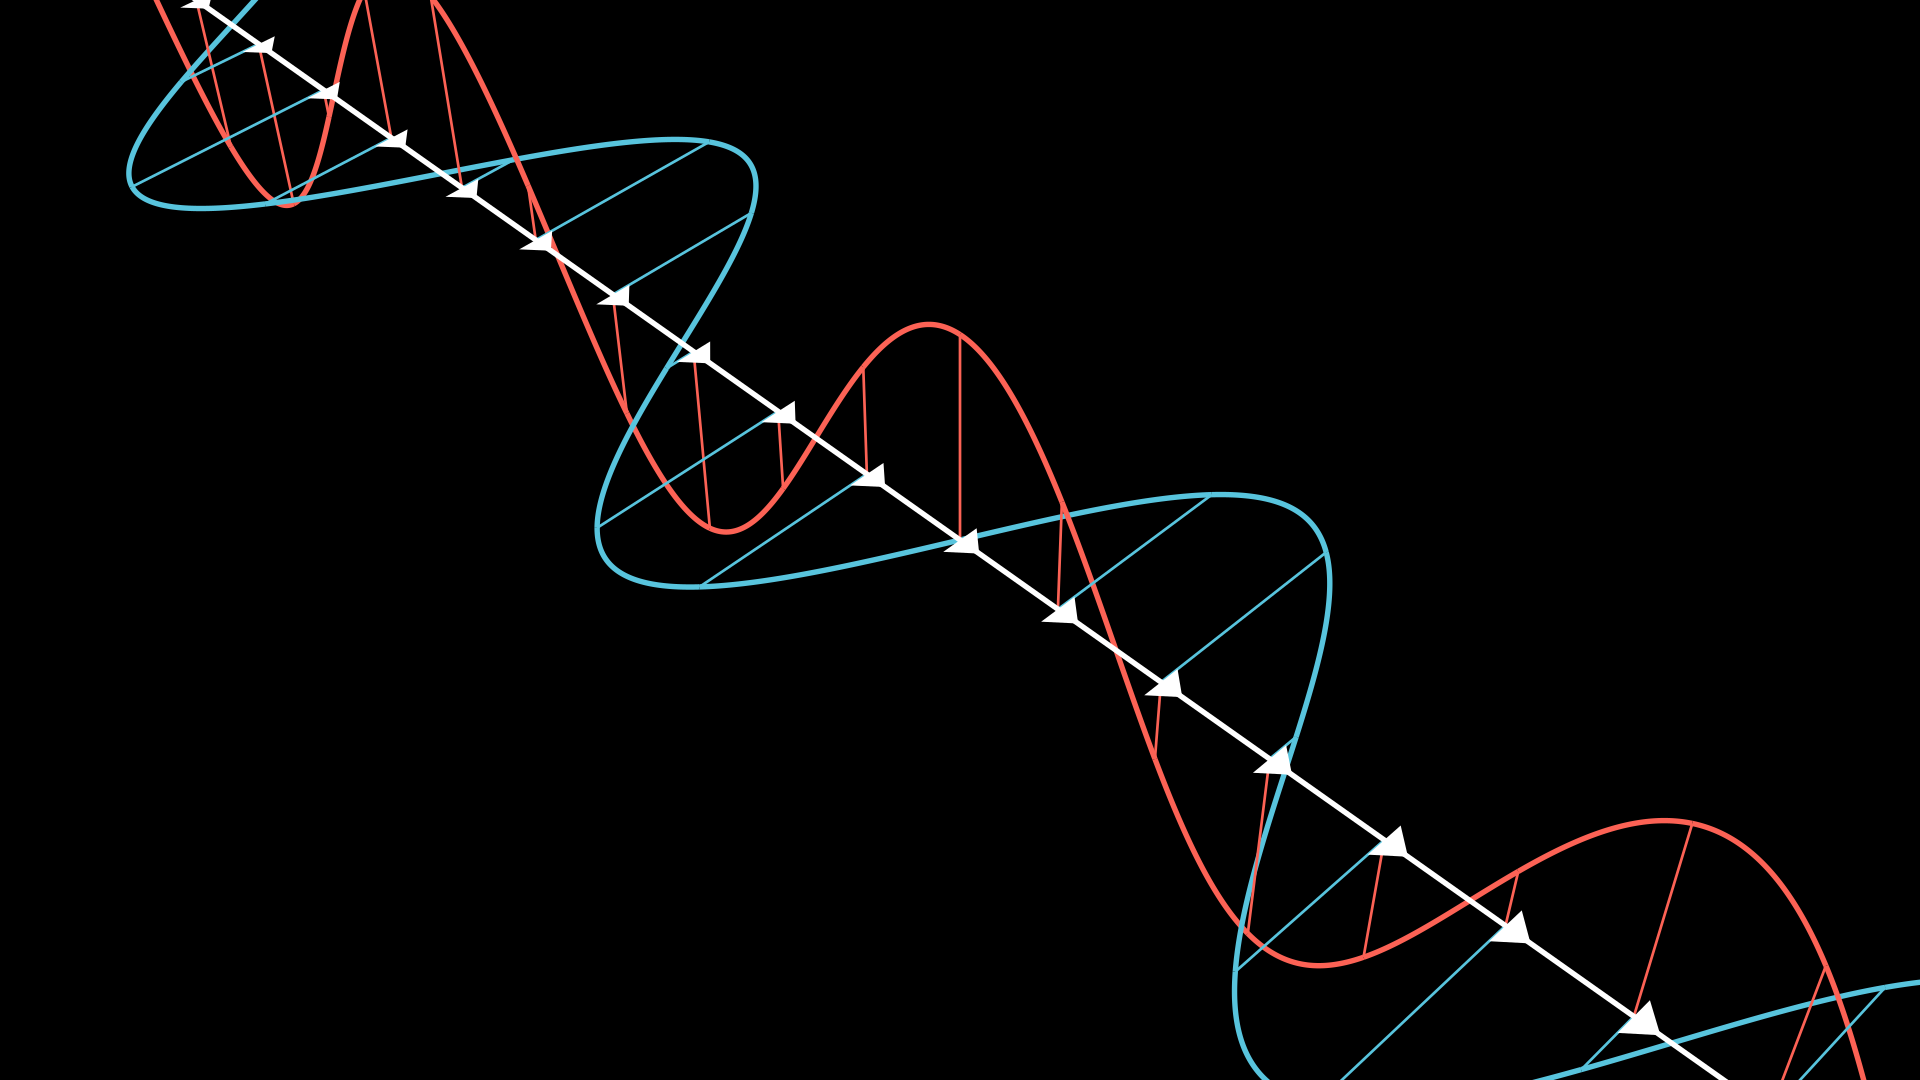
\includegraphics[width=\textwidth]{electromagnetic_wave.png}
    \caption{Representación de una onda electromagnetica propagandose por el espacio}
    \label{fig:electromagnetic-wave}
\end{figure}

A principios del siglo XX, los trabajos liderados por Max Planck, Max Born, Erwin Schrödinger, y Werner Heisenberg condujeron a otro cambio sustancial en el entendimiento de la luz.
A nivel microscópico, las propiedades elementales como energía y momento solo pueden existir como un múltiplo entero de una cantidad base conocida como un \textbf{cuanto}.
En el caso de oscilaciones electromagnéticas, este cuanto se conoce como \textbf{fotón}.
La luz existe tanto como onda y como partícula \cite{quantum-light}.

Afortunadamente, el complejo comportamiento de onda de la luz aparece en escalas muy pequeñas, por lo que, para la computación gráfica, en la mayoría de los casos, se la puede tratar como partícula.
Esto simplifica los cálculos \cite{pbr}.

Tratar a la luz como una partícula es el campo de la óptica geométrica, en contraposición a la óptica física.
La óptica geométrica trata a la luz como rayos que se mueven en líneas rectas.
La óptica física aborda la luz desde el punto de vista de su naturaleza ondulatoria, centrándose en fenómenos como la interferencia, la difracción, la polarización.
Si asumimos que las irregularidades de las superficies son en general mucho más grandes que la longitud de onda de la luz, estos efectos no ocurren, y se puede tratar la luz como rayos \cite{rtr}.
Esto remueve otros fenómenos como la fluorescencia, la fosforescencia y la polarización.

% Esto asume varias otras cosas, como linealidad, conservación de la energía, falta de polarización, fluorescencia y fosforescencia, entre otros.

\section{Radiometría: Unidades de la luz}\label{sec:radiometry}

La radiometría provee una serie de herramientas para describir la propagación de la luz.
Para simular luz, es necesario un manejo de las unidades básicas involucradas.
Algunas de estas son la energía radiante, el flujo radiante, la radiosidad, la irradiancia, la intensidad radiante, y la radiancia.
La descripción de estas unidades surgen de \cite{rtr} y \cite{pbr}.

La \textbf{energía radiante} es la energía de la radiación electromagnética de la luz.
Se mide en joules y se denota con el símbolo $Q$.
Las fuentes de iluminación emiten fotones, y cada uno posee una longitud de onda y una energía particular.
Un fotón con longitud de onda $\lambda$ tiene una energía $Q = \frac{hc}{\lambda}$, donde $c$ es la velocidad de la luz y $h$ es la constante de Planck, el cuanto.

El \textbf{flujo radiante}, o potencia, es la energía que pasa por una superficie o región del espacio por unidad de tiempo: $\Theta = \frac{dQ}{dt}$.
Se mide en joules por segundo, o watts.
En la figura \ref{fig:point-light-flux} se representa en 2D una luz puntual emitiendo fotones en todas las direcciones.
Los círculos de la figura son áreas en las que se mide el flujo radiante que pasa por ellas.
Por cada círculo pasa el mismo flujo radiante, dado que la energía y el tiempo son los mismos.

\begin{figure}[ht]
    \centering
    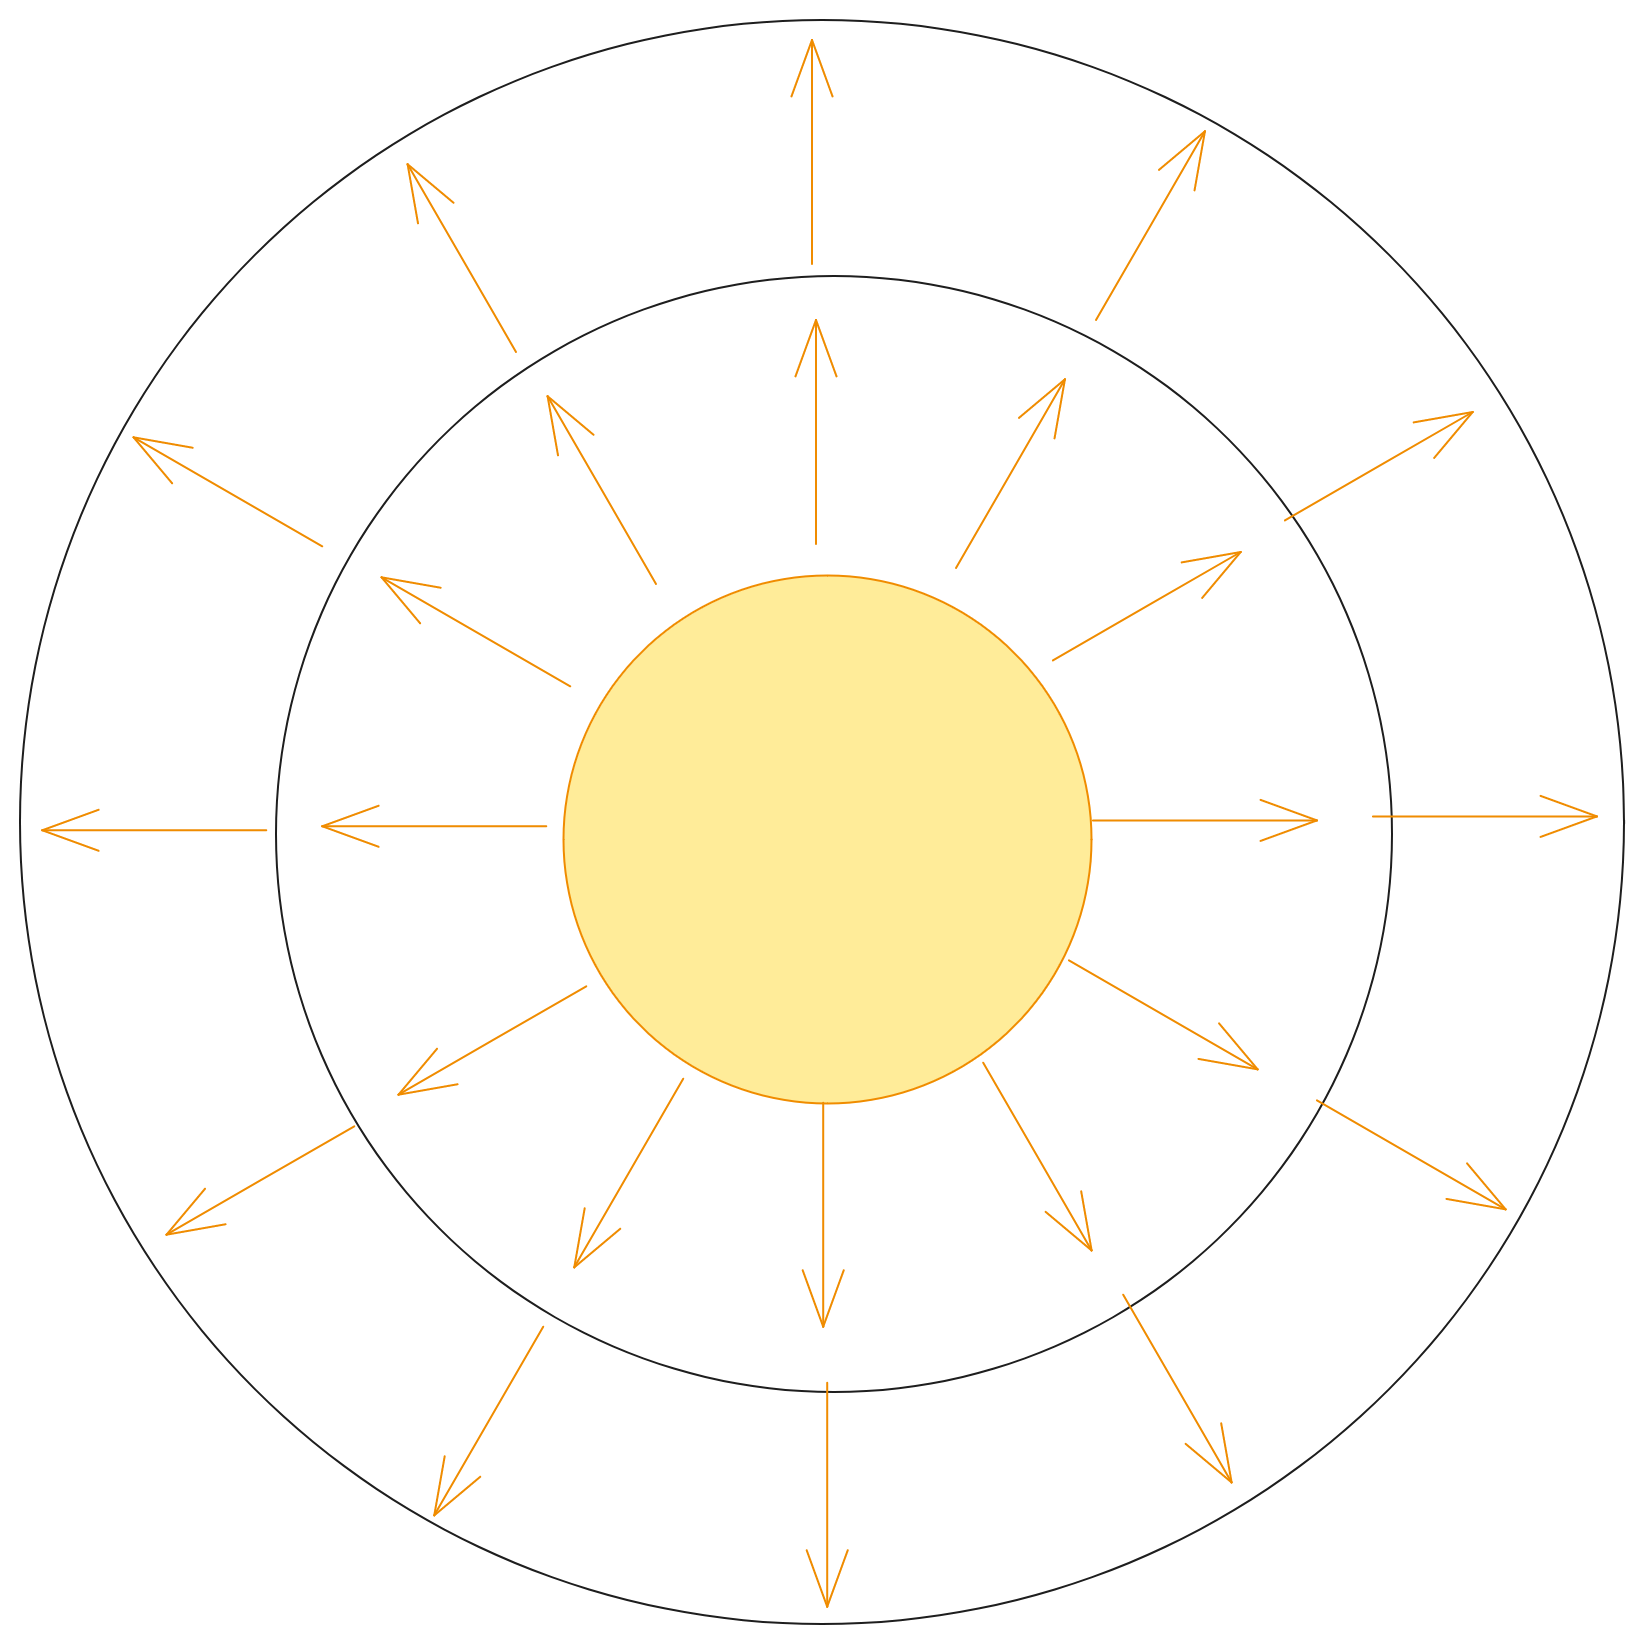
\includegraphics[width=0.25\textwidth]{point-light-flux.png}
    \caption{Flujo radiante en una luz puntual}
    \label{fig:point-light-flux}
\end{figure}

Es útil también considerar el área por la cual pasa un flujo radiante.
Podemos definir esto como $E = \frac{\Theta}{A}$.
Esta cantidad se llama o \textbf{radiosidad} o \textbf{irradiancia} dependiendo de si el flujo está llegando o saliendo de una superficie.
Estas medidas tienen unidad watts por metro cuadrado.
En la figura \ref{fig:point-light-flux}, la irradiancia en el círculo externo es menor que en el interno, dado que el área aumenta cuadráticamente con la distancia.

Para definir la próxima unidad, es necesario definir el \textbf{ángulo sólido}, que es la extensión a 3D del ángulo bidimensional.
En 2D, un ángulo mide el tamaño de un conjunto continuo de direcciones en un plano.
Para medir esto, se mide el largo del arco resultante de la intersección de este conjunto con un círculo de radio 1.
El largo de este arco se mide en radianes.
De igual manera, un ángulo sólido mide el tamaño de un conjunto de direcciones en el espacio.
Para lograr esto, se mide el área de la intersección del conjunto de direcciones con una esfera de radio 1.
La unidad de medida es el estereorradián.
El ángulo sólido se representa con el símbolo $\omega$.
En la figura \ref{fig:steradian} se puede ver un cono con un ángulo sólido de 1 estereorradián.
El ángulo sólido que abarca todas las direcciones posibles mide $4\pi$ estereorradianes.

\begin{figure}[ht]
    \centering
    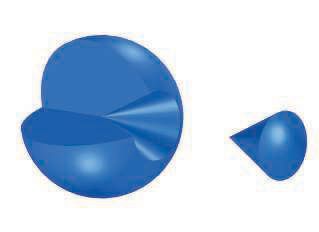
\includegraphics[width=0.4\textwidth]{steradians.png}
    \caption{Un cono con un ángulo sólido de 1 estereorradián removido de una esfera. Fuente: \cite{rtr}}
    \label{fig:steradian}
\end{figure}

La \textbf{intensidad radiante} es el flujo radiante dada una dirección, o mejor dicho, un ángulo sólido.
Se denota $I(\omega) = \frac{d\Theta}{d\omega}$ y se mide en watts por estereorradián.

Llegamos a la unidad radiométrica más importante, la \textbf{radiancia}.
La radiancia es la cantidad de flujo radiante emitida, reflejada, transmitida o recibida por una superficie por unidad de área y por unidad de ángulo sólido.
Se denota como $L$ y se mide en watts por metro cuadrado por estereorradián.

$$
L = \frac{d^2\Theta}{(dA\,\cos\theta)d\omega}
$$

La radiancia es lo que miden los sensores, como los ojos o cámaras.
El objetivo de evaluar una ecuación de sombreado es calcular la radiancia a lo largo de un rayo, desde el punto de vista de la cámara.

Lo anteriormente expuesto son algunas unidades de la radiometria que trata unicamente con cantidades fisicas de la luz.
En contraposicion, un campo relacionado, la fotometría mide la luz en funcion de la percepcion del ojo humano.

La radiometría trata únicamente con cantidades físicas de la luz.
En contraposición, un campo relacionado, la fotometría, mide la luz tal como es percibida por el ojo humano, teniendo en cuenta la sensibilidad de este a distintas longitudes de onda.
En la tabla \ref{table:light_units} se muestran algunas unidades equivalentes en radiometría y fotometría.

\begin{table}
\centering
\begin{tabular}{|c|c|}
    \hline
    \textbf{Radiometría (unidad)} & \textbf{Fotometría (unidad)} \\
    \hline
    Flujo radiante ($W$) & Flujo luminoso ($lumen, lm$) \\
    \hline
    Radiosidad $\left(\frac{W}{m^2}\right)$ & Emitancia luminosa $\left(\frac{lm}{m^2} = lux, lx\right)$ \\
    \hline
    Irradiancia $\left(\frac{W}{m^2}\right)$ & Iluminancia ($lx$) \\
    \hline
    Intensidad radiante $\left(\frac{W}{sr}\right)$ & Intensidad luminosa ($candela, cd$) \\
    \hline
    Radiancia $\left(\frac{W}{(m^2sr)}\right)$ & Luminancia $\left(\frac{cd}{m^2} = nit\right)$ \\
    \hline
\end{tabular}
\caption{Unidades de radiometría y fotogrametría}
\label{table:light_units}
\end{table}

\section{Iluminación local e iluminación global}\label{sec:local_vs_global}

En computación gráfica, la iluminación es crucial para agregar realismo a una escena, sin embargo, es también uno de los aspectos más desafiantes desde el punto de vista computacional, debido a la complejidad de simular cómo la luz interactúa con los objetos y el entorno.

\subsection{Iluminación local}

La iluminación local es un enfoque más simple y menos demandante computacionalmente, que ayuda a dar una sensación de tridimensionalidad.
Consiste en calcular la iluminación directa para cada objeto individualmente, sin considerar la iluminación indirecta que existe entre objetos vecinos.
Al no calcular la interacción de la luz con otros objetos, se simplifican significativamente los cálculos necesarios para generar la imagen.

Sus ventajas son su simplicidad y su eficiencia.
Su mayor desventaja es que no abarca fenómenos como la refracción, las cáusticas y el sangrado, entre otros.

Un modelo ampliamente utilizado para iluminación local es el de Blinn-Phong, \cite{blinn-phong}.
Este posee tres componentes principales: luz \textbf{ambiente}, \textbf{difusa} y \textbf{especular}.
La luz ambiente es uniforme y está presente en toda la escena.
No proviene de una fuente de luz en particular y simula el efecto de la luz indirecta que proviene del resto de la escena.
La luz difusa representa el efecto de la luz directa que incide sobre una superficie rugosa y se refleja en todas las direcciones.
Depende del ángulo entre la dirección de la luz y la normal de la superficie.
La luz especular simula el brillo que se ve cuando la luz se refleja sobre superficies pulidas.
Este componente depende de la dirección de vista, de la normal de la superficie y de la dirección de la fuente luminosa en cada punto de la superficie.

% TODO: Fotos, ambiente, difusa, especular y todo junto

\begin{figure}
    \begin{center}

    \begin{subfigure}{.24\textwidth}
        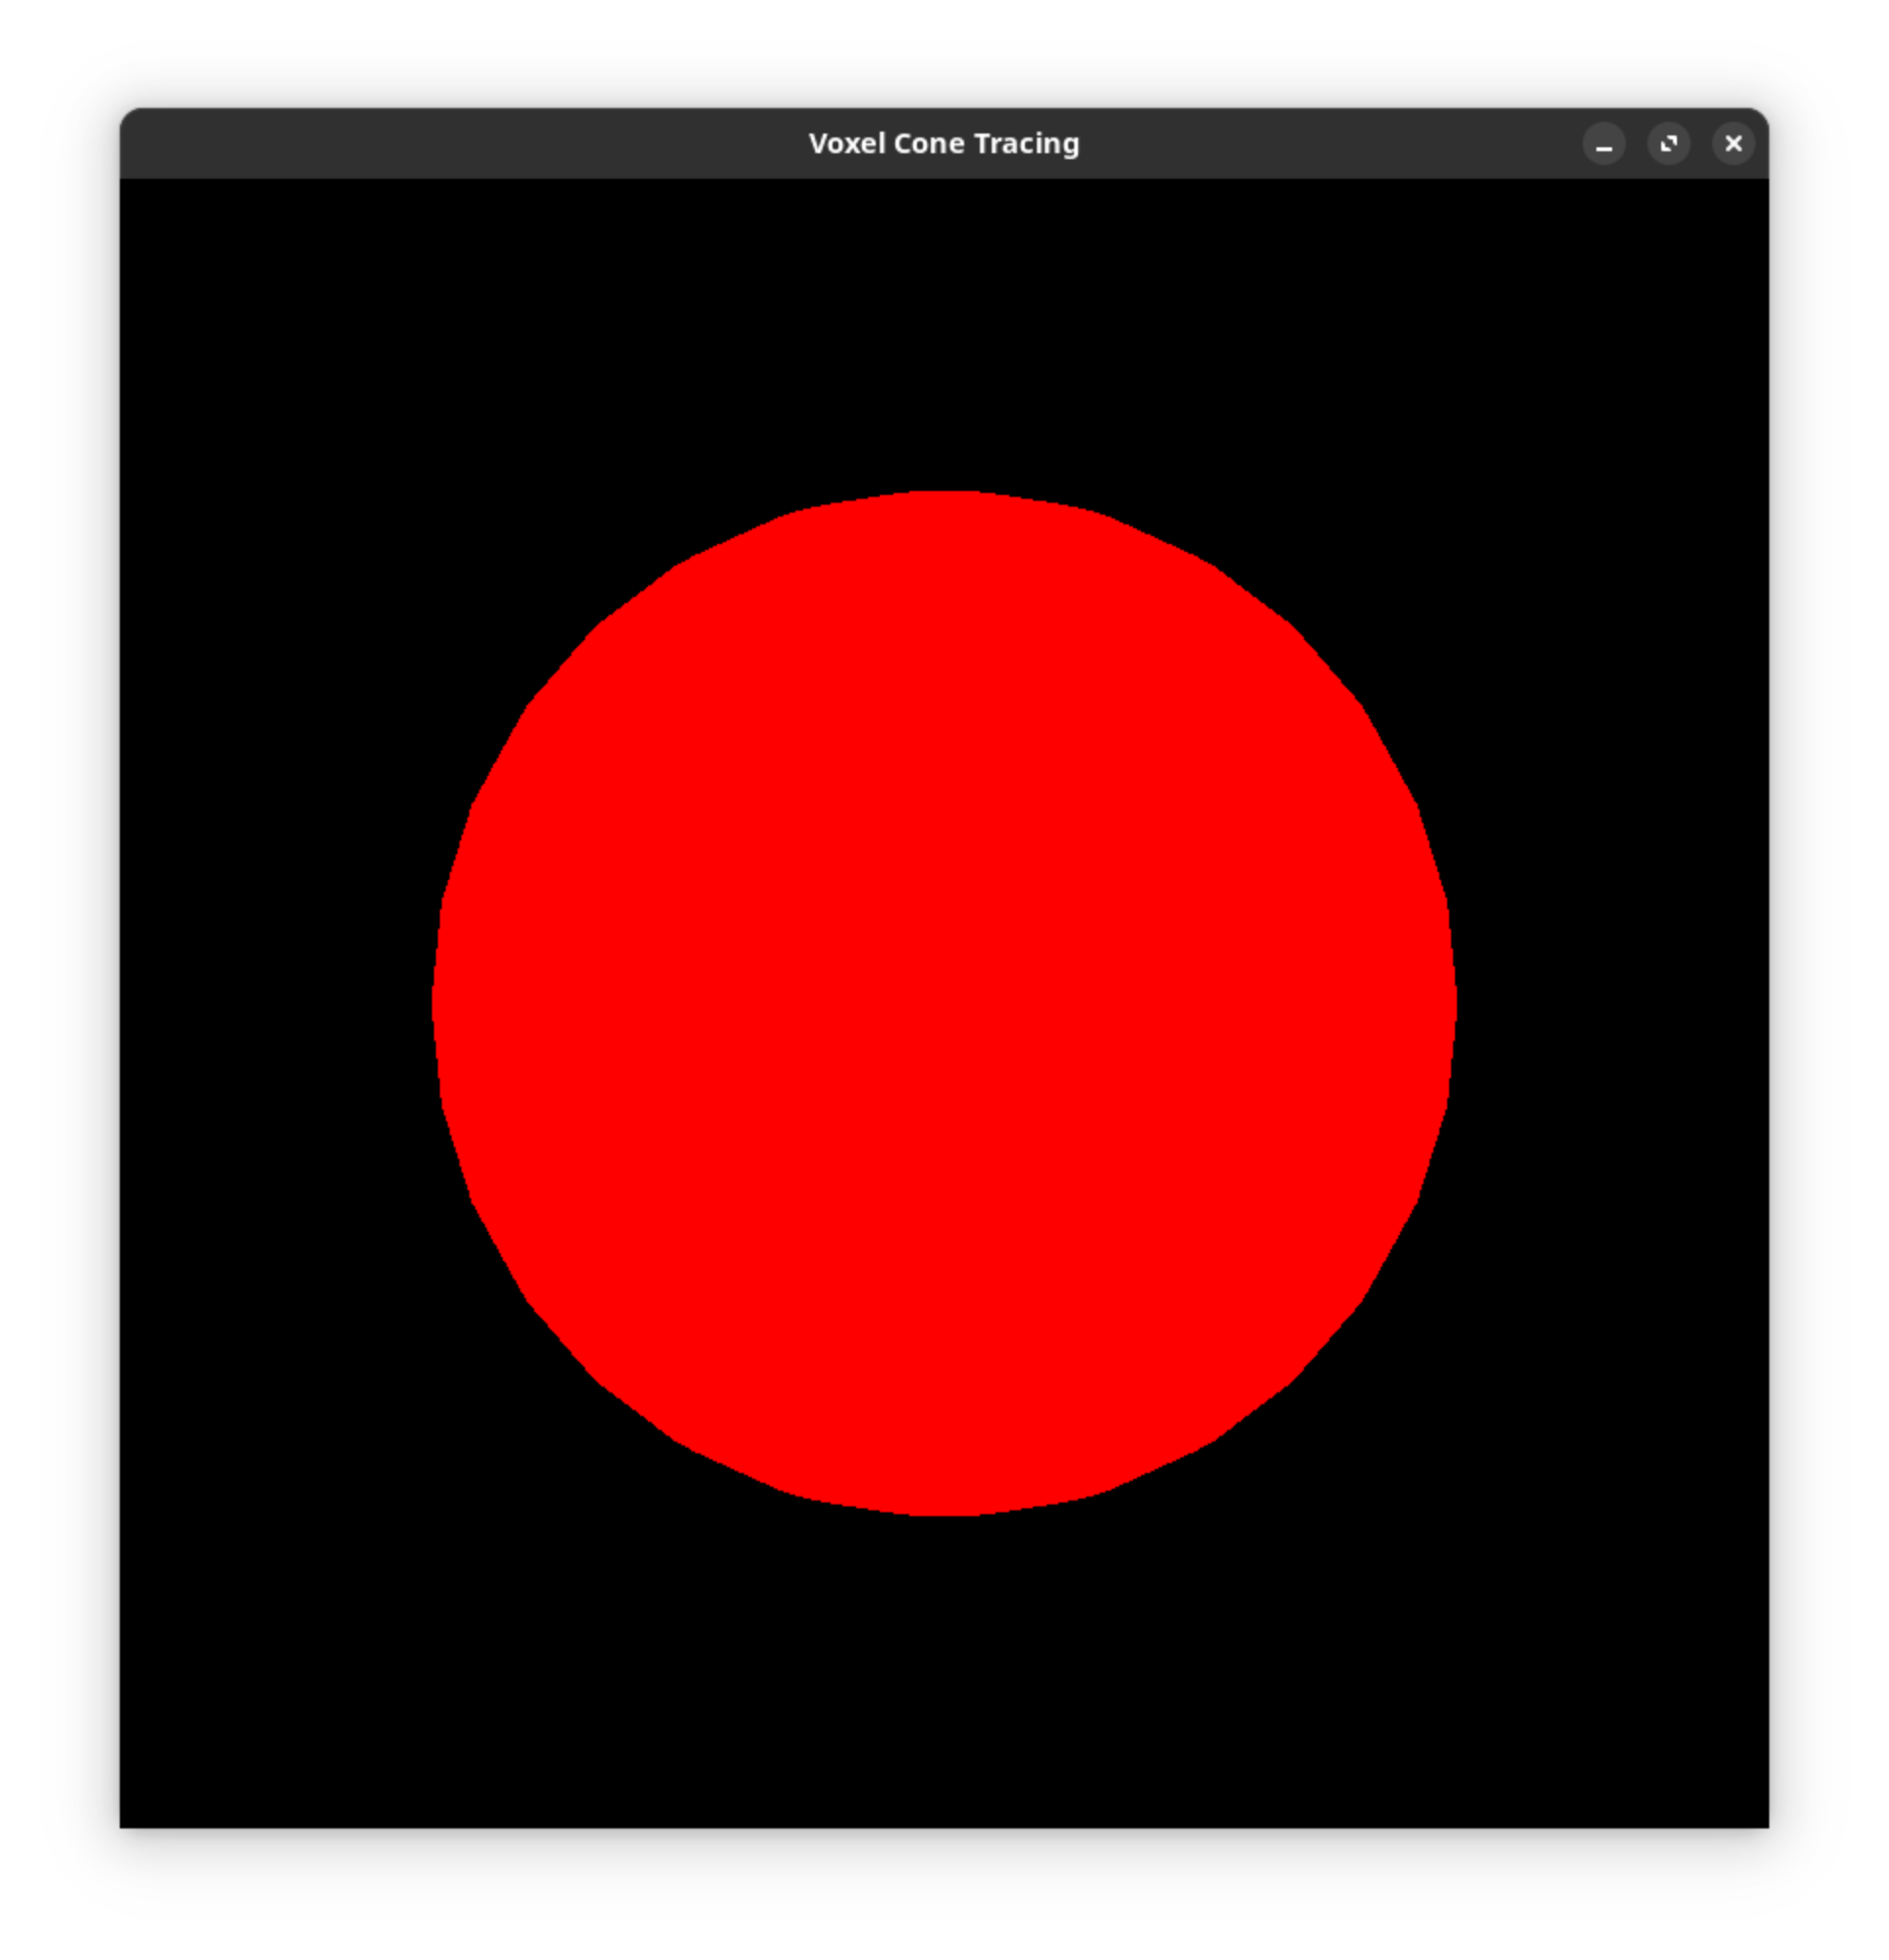
\includegraphics[width=\textwidth]{sphere-unshaded.png}
        \caption{Sin sombreado}
    \end{subfigure}

    \begin{subfigure}{.24\textwidth}
        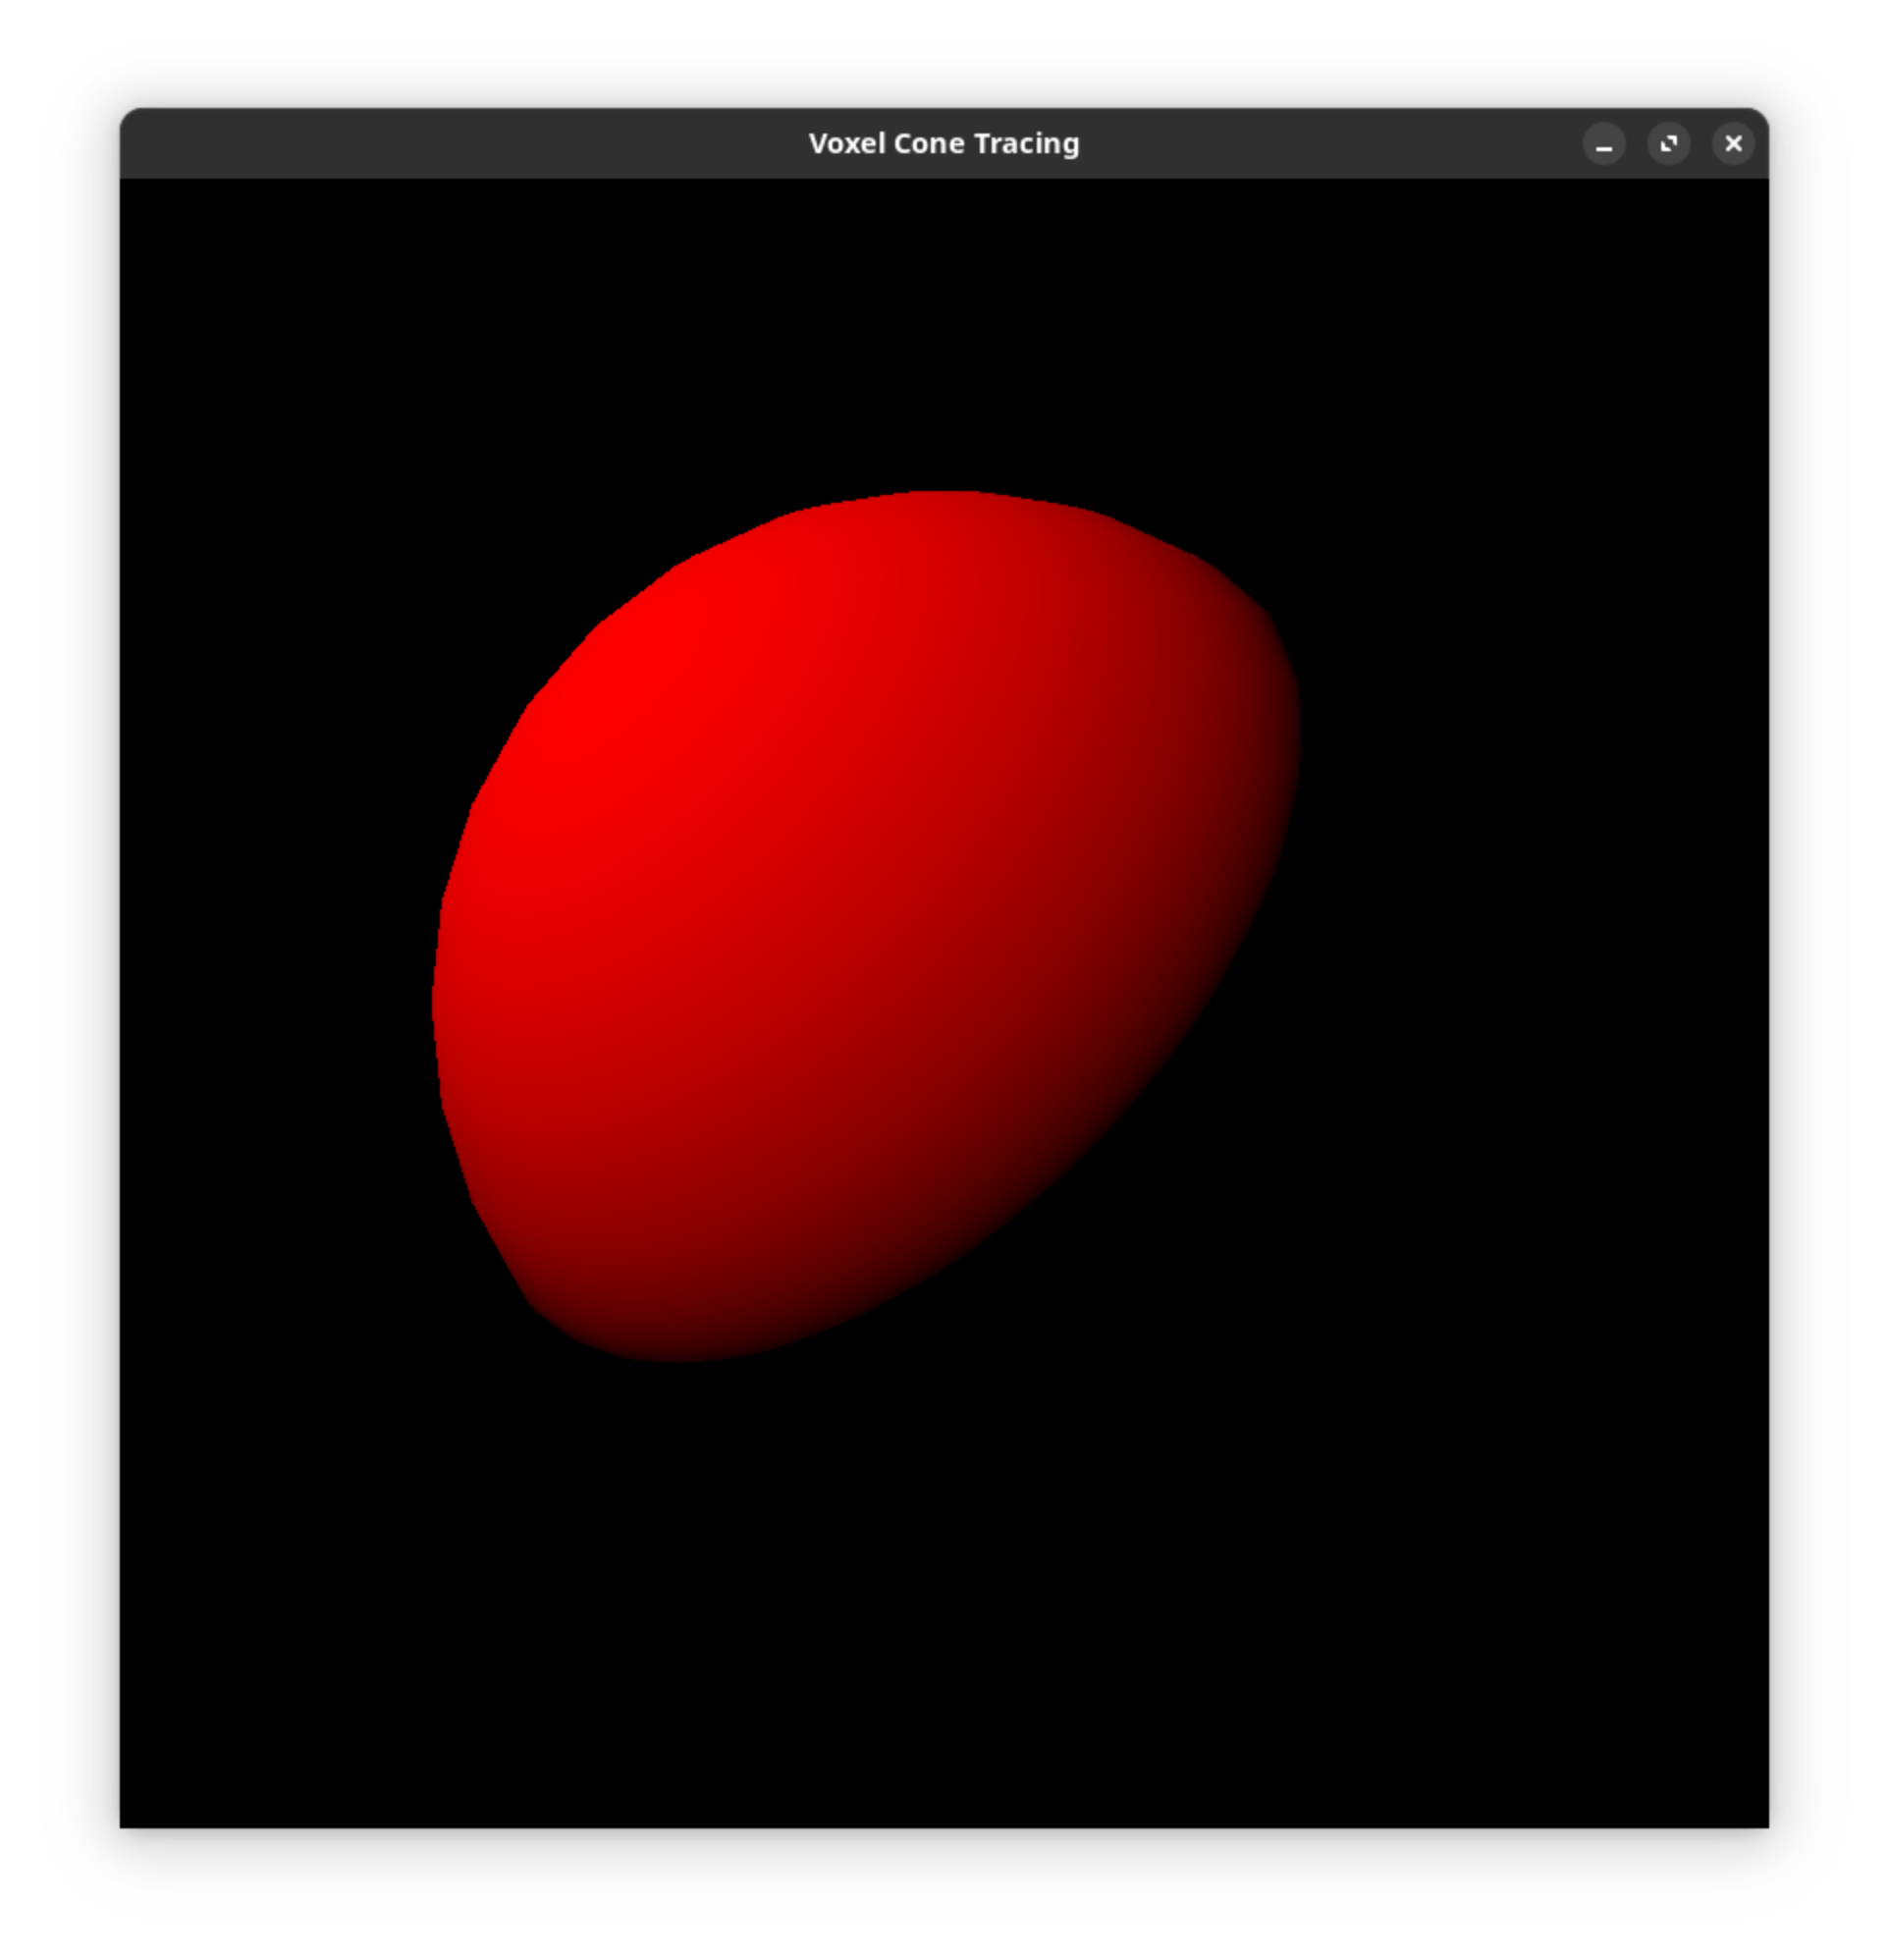
\includegraphics[width=\textwidth]{sphere-diffuse.png}
        \caption{Con sombreado difuso}
    \end{subfigure}

    \end{center}

    \caption{Esfera iluminada mediante el módelo local de Blinn-Phong}
    \label{fig:sphere-blinn-phong}
\end{figure}

\subsection{Iluminación global}

En contraposición a la iluminación local, la iluminación global calcula la interacción completa de la luz con los objetos de la escena.
Se calcula la interacción de la luz entre distintos objetos al reflejarse, refractarse y dispersarse en el entorno.

Su principal ventaja es la mejora en el realismo y coherencia de la escena, mientras que su principal desventaja es la exigencia computacional y complejidad al implementar y optimizar.
Esto causa que sea difícil alcanzar tiempos interactivos.

Entre las técnicas más utilizadas se encuentra el trazado de rayos, la radiosidad, el \textit{photon mapping}, y el \textit{path tracing}, que serán presentadas a continuación.

En 1986, James T. Kajiya presentó la \textbf{ecuación de renderizado}, formalizando varios métodos para el cálculo de iluminación global como aproximaciones a la solución de una misma ecuación, \cite{rendering-equation}:

\begin{equation}\label{eq:rendering-equation}
    I(x, x') = g(x, x') \cdot \left[\epsilon(x, x') + \int_S f(x, x', x'') \cdot I(x', x'') \cdot dx'' \right]
\end{equation}

donde:
\begin{itemize}
    \item $I(x, x')$ se relaciona con al intensidad radiante que pasa del punto $x'$ al punto $x$.
    \item $g(x, x')$ es un término de "geometría", evalúa si hay algo interponiéndose en el camino de $x'$ a $x$.
    \item $\epsilon(x, x')$ se relaciona con la intensidad emitida desde $x'$ en dirección a $x$.
    \item $f(x, x', x'')$ es la función de distribución de reflectancia bidireccional (BRDF, por sus siglas en inglés). Se relaciona con la intensidad de luz reflejada desde $x''$ hacia $x$ a través de $x'$. En la sección \ref{sec:brdf} se analizan casos particulares de esta función.
    \item $S = \cup{S_i}$, el dominio de la integral, es la unión de todas las superficies de la escena. Esto significa que los puntos $x, x', x''$ varían a lo largo de todas las superficies.
\end{itemize}

En palabras, la ecuación \ref{eq:rendering-equation} establece que la intensidad que llega a un punto $x$ desde otro punto $x'$, es la intensidad que $x'$ emite en dirección a $x$ más la intensidad reflejada por $x'$ hacia $x$ desde cualquier otro punto de la escena.
Todo sujeto a si hay geometría en el camino de $x$ a $x'$, si es que $x'$ ``ve'' a $x$.

Los términos ``intensidad radiante'' e ``intensidad emitida'' tal y como son planteados no son exactamente ninguna de las unidades radiométricas vistas en la sección \ref{sec:radiometry} pero son cantidades que pueden derivarse de estas.

Esta ecuación es la base de varios métodos de iluminación global \cite{rtr}.
Se puede observar que esta ecuación tiene en cuenta toda la escena para calcular la luz en un punto.

La ecuación no presenta una solución analítica cerrada para la mayoría de los casos, por lo que se calculan soluciones numéricas para su resolución.

La ecuación \ref{eq:rendering-equation} considera toda la iluminación de la escena, incluyendo tanto luz directa como indirecta.
La \textbf{ecuación de reflectancia} se deriva de la de renderizado y se enfoca en el cálculo de la luz indirecta.

\begin{equation}\label{eq:reflectance-equation}
    L_o(p, \omega_o) = \int_{\Omega}{f(p, \omega_i, \omega_o) L_i(p, \omega_i) n \cdot \omega_i d\omega_i}
\end{equation}

Esta ecuación calcula la radiancia saliente $L_o$ de un punto $p$ y un pequeño ángulo sólido $\omega_o$ como una integral sobre el hemisferio $\Omega$ centrado en el punto.
Sus términos son muy parecidos a los de la ecuación de renderizado.
Vemos que ya no están el término geométrico, dado que se trata de direcciones y no puntos, ni el término de emisión, dado que solo se considera luz indirecta.
$f$ es la BRDF.
$L_i(p, \omega_i)$ es la radiancia entrante hacia $p$ por otra dirección $\omega_i$.
$n$ es la normal en el punto $p$ y $n \cdot \omega_i$ es el producto interno entre la normal y la dirección, que equivale al coseno del ángulo entre ellos.
La radiancia saliente es la suma por todo el hemisferio $\Omega$ centrado en $p$.
La suma de todas las radiancias a lo largo del hemisferio es la irradiancia, como se vió anteriormente.

% \begin{figure}
%     \centering
%     \includegraphics[width=\textwidth]{}
%     \caption{Hemisferio centrado en un punto $p$}
%     \label{fig:hemisphere}
% \end{figure}

\section{BRDF}\label{sec:brdf}

La \textbf{función de distribución de reflectancia bidireccional} (BRDF, por sus siglas en inglés), es una función $f(x, \omega, \omega')$ que dado un punto $x$, una dirección $\omega$ entrante y una saliente $\omega'$, retorna cuánta luz se refleja desde la dirección entrante hacia la saliente en el punto.

Está función se puede obtener usando tanto modelos analíticos como midiendo objetos reales con cámaras calibradas y fuentes de luz.
A lo largo de los años, se han propuesto varios BRDFs, tanto teóricos como empíricos \cite{review-of-brdf-models}.
Los BRDFs son propios de los materiales, y este es uniforme a lo largo de todo el material, por lo que no se diferencia entre dos puntos distintos $x$ y $x'$ del mismo material.

% TODO: Agregar una foto de la máquina utilizada para medir BRDFs
% TODO: Podemos hablar más de cómo se representan capaz

Dos casos teóricos e ideales son los siguientes:

\begin{itemize}
    \item Reflexión especular: $f(x, \omega, \omega') = \rho$ cuando $\omega$ es simétrico a $\omega'$ respecto a la normal. $0$ en otro caso.
    \item Reflexión difusa: $f(x, \omega, \omega') = \frac{\rho}{\pi}$ para todas las direcciones donde $\rho$ es la reflectividad de la superficie, es decir, la fracción de la energía reflejada con respecto a la energía incidente total.
\end{itemize}

La reflexión especular refleja un rayo solamente en un ángulo específico.
La reflexión difusa refleja la luz igual en todas las direcciones, con un mismo valor de BRDF para cada una de ellas.

Estos BRDFs son muy utilizados, dado que simplifican mucho los calculos y son fisicamente posibles, aunque no existan materiales reales con estas características de reflectancia.

\section{Trazado de rayos (\textit{ray tracing})}\label{sec:ray-tracing}

Uno de los métodos más antiguos y populares para calcular la iluminación global es el de trazado de rayos.
Este se basa en tratar a la luz como una partícula, y trazar el camino que toman los rayos de luz a través de la escena, calculando reflección, refracción y absorción del rayo cuando interseca con un objeto.
La popularidad de este método surge debido a su simplicidad y al gran realismo que agrega a las imágenes generadas.
Su primer uso como herramienta de computación gráfica para representar reflexión, refracción y sombras se atribuye a Turner Whitted, en 1980, \cite{whitted-1980}.

\textit{Ray tracing} lanza rayos desde la cámara a través de la grilla de píxeles hacia la pantalla.
Por cada rayo, se busca la intersección con el objeto más próximo.
El punto de intersección se prueba si está en sombra lanzando un nuevo rayo hacia todas las luces de la escena y comprobando si se intersecan con algún objeto.
Pueden surgir otros rayos desde la intersección.
Si la superficie es especular, se genera un rayo en la dirección simétrica a la dirección de vista.
Si la superficie es transparente, se genera un rayo en la dirección de refracción, gobernada por la ley de Snell\footnote{$n_1 \sin{\theta_1} = n_2 \sin{\theta_2}$}.
En la figura \ref{fig:whitted-ray-tracing} se puede ver una imagen generada por este método.

Este método sufre de \textit{aliasing}, los bordes irregulares.
Esto ocurre debido a una falta de resolución, es decir, cantidad de píxeles, que no logra capturar todo el detalle de la imagen.
Suele notarse al representar curvas.
Se puede ver en la figura \ref{fig:whitted-ray-tracing}.

% TODO: Agregar diagramas de 1) sombra, 2) reflexión y 3) refracción.

\begin{figure}
    \begin{center}
    \begin{subfigure}{.69\textwidth}
        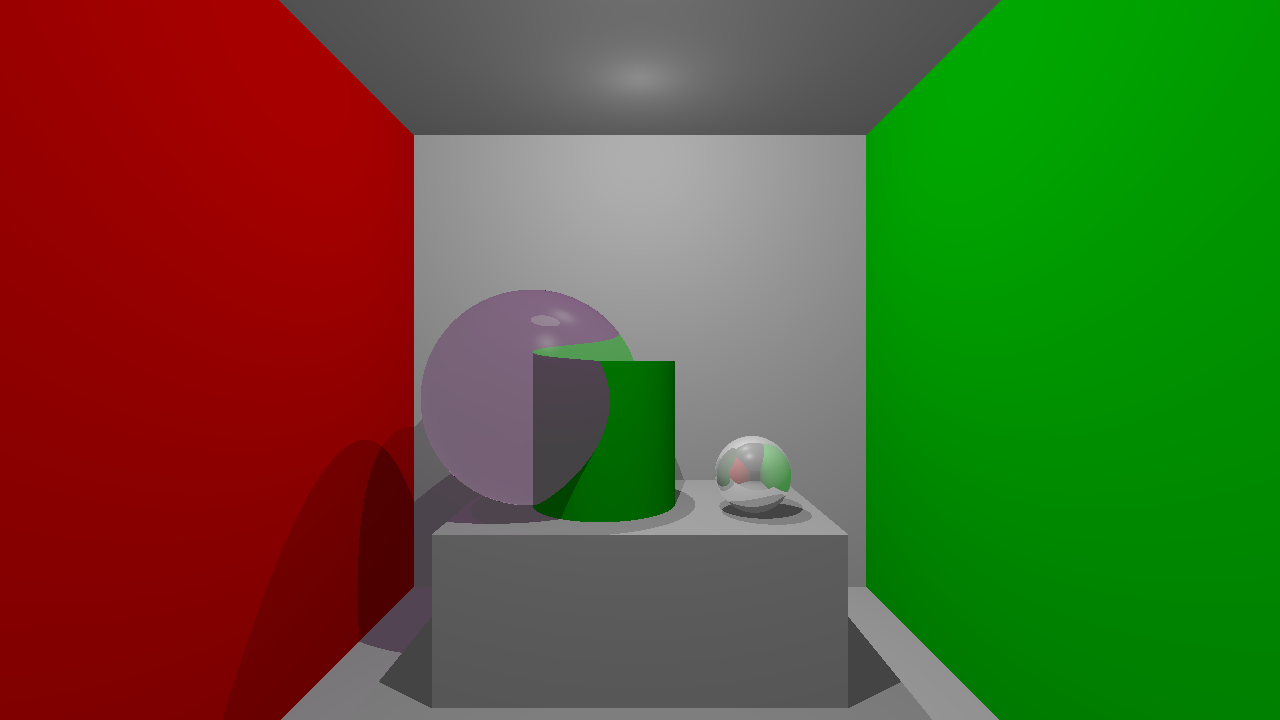
\includegraphics[width=\textwidth]{whitted-ray-tracing.png}
        \caption{Escena entera}
    \end{subfigure}
    \begin{subfigure}{.3\textwidth}
        
\includegraphics[width=\textwidth]{whitted-aliasing.png}
        \caption{\textit{Aliasing}}
    \end{subfigure}
    \caption{Escena renderizada con el trazado de rayos de Whitted. Implementación propia.}
    \label{fig:whitted-ray-tracing}
    \end{center}
\end{figure}

Kajiya propuso en 1986\cite{rendering-equation}, junto con la ecuación de renderizado, un método llamado \textit{path tracing}, una extensión de \textit{ray tracing} que utiliza integración de Monte Carlo para simular la dispersión de la luz.
En lugar de únicamente trazar los caminos de reflexión y refracción si corresponden, muestrea aleatoriamente todos los posibles caminos de la luz, esto incluye caminos en los que la luz se dispersa.
Es imposible muestrear todos los caminos posibles de la luz, por lo que un parámetro importante en este tipo de algoritmos es la cantidad de muestras que se toman.
Debido a la variancia del muestreo aleatorio, este método sufre de ruido, un granulado en la imagen final.
El mismo disminuye a medida que se toman más muestras.

% TODO: Imagen generada con path tracing y ruido

Tanto el \textit{aliasing} como el ruido pueden mitigarse con una técnica llamada \textit{supersampling}.
Consiste en tomar más de una muestra por píxel, lo que significa lanzar más de un rayo por píxel y luego promediar los resultados.
Esto suaviza las curvas, mitigando el \textit{aliasing}, y provee más muestras aleatorias para la integración de Monte Carlo, lo que reduce el ruido.
Es una técnica muy costosa dado que implica lanzar cantidades mucho mayores de rayos.
Para imágenes complejas, pueden ser necesarios cientos de rayos por píxel para reducir el ruido a niveles aceptables.
Esto imposibilita la generación de imágenes en tiempo real.
Debido a la complejidad computacional agregada por esta técnica, han surgido otras.
La estrella de las técnicas de reducción de ruido son los \textit{denoisers} basados en el uso de redes neuronales.
% TODO: Referenciasss

Varios métodos de iluminación global basados en el trazado de rayos han surgido desde entonces.

\section{Trazado de conos}\label{sec:historical-cone-tracing}

En su artículo de 1984 \cite{ray-tracing-with-cones}, Amanatides propone una extensión al trazado de rayos en la que redefine los rayos por conos.
Los rayos tienen un origen, una dirección y son infinitesimalmente finos.
Los conos tienen a su vez un ángulo de apertura, lo cual agrega un grosor no despreciable.
Usando este grosor, los conos son capaz de no solo probar la existencia de intersecciones, sino también calcular el porcentaje de área de la intersección.
Este método fue propuesto para solucionar el \textit{aliasing} presente en el trazado de rayos, como alternativa al \textit{supersampling}.
En lugar de lanzar muchos rayos por cada píxel, se lanza un solo cono que integra una mayor área de la escena.
Dado que el cono tiene en cuenta la contribución de la luz de varias direcciones dentro de su volumen, reduce el \textit{aliasing} y el ruido al muestrear mayor parte de la escena y reducir la variancia del muestreo.

Esta idea de trazar conos en lugar de rayos no solo ayuda en el \textit{aliasing} y el ruido.
También permite generar sombras suaves.
En el trazado de rayos, al probar si un punto se encuentra en sombra o no, se lanza un rayo hacia la fuente de la luz.
Si este interseca con algún objeto antes de llegar a la luz, el punto está en sombra.
Esta respuesta binaria, si o no, a la pregunta de si el punto se encuentra en sombra resulta en sombras duras.
Al trazar un cono en lugar de un rayo hacia la fuente de luz, es posible responder el porcentaje de oclusión de ese punto, lo cual lleva a una escala de grises y a sombras suaves.
En la figura \ref{fig:shadow-rays-and-cones} se pueden ver diagramas mostrando esta diferencia.

\begin{figure}
    \begin{center}
    \begin{subfigure}{.49\textwidth}
        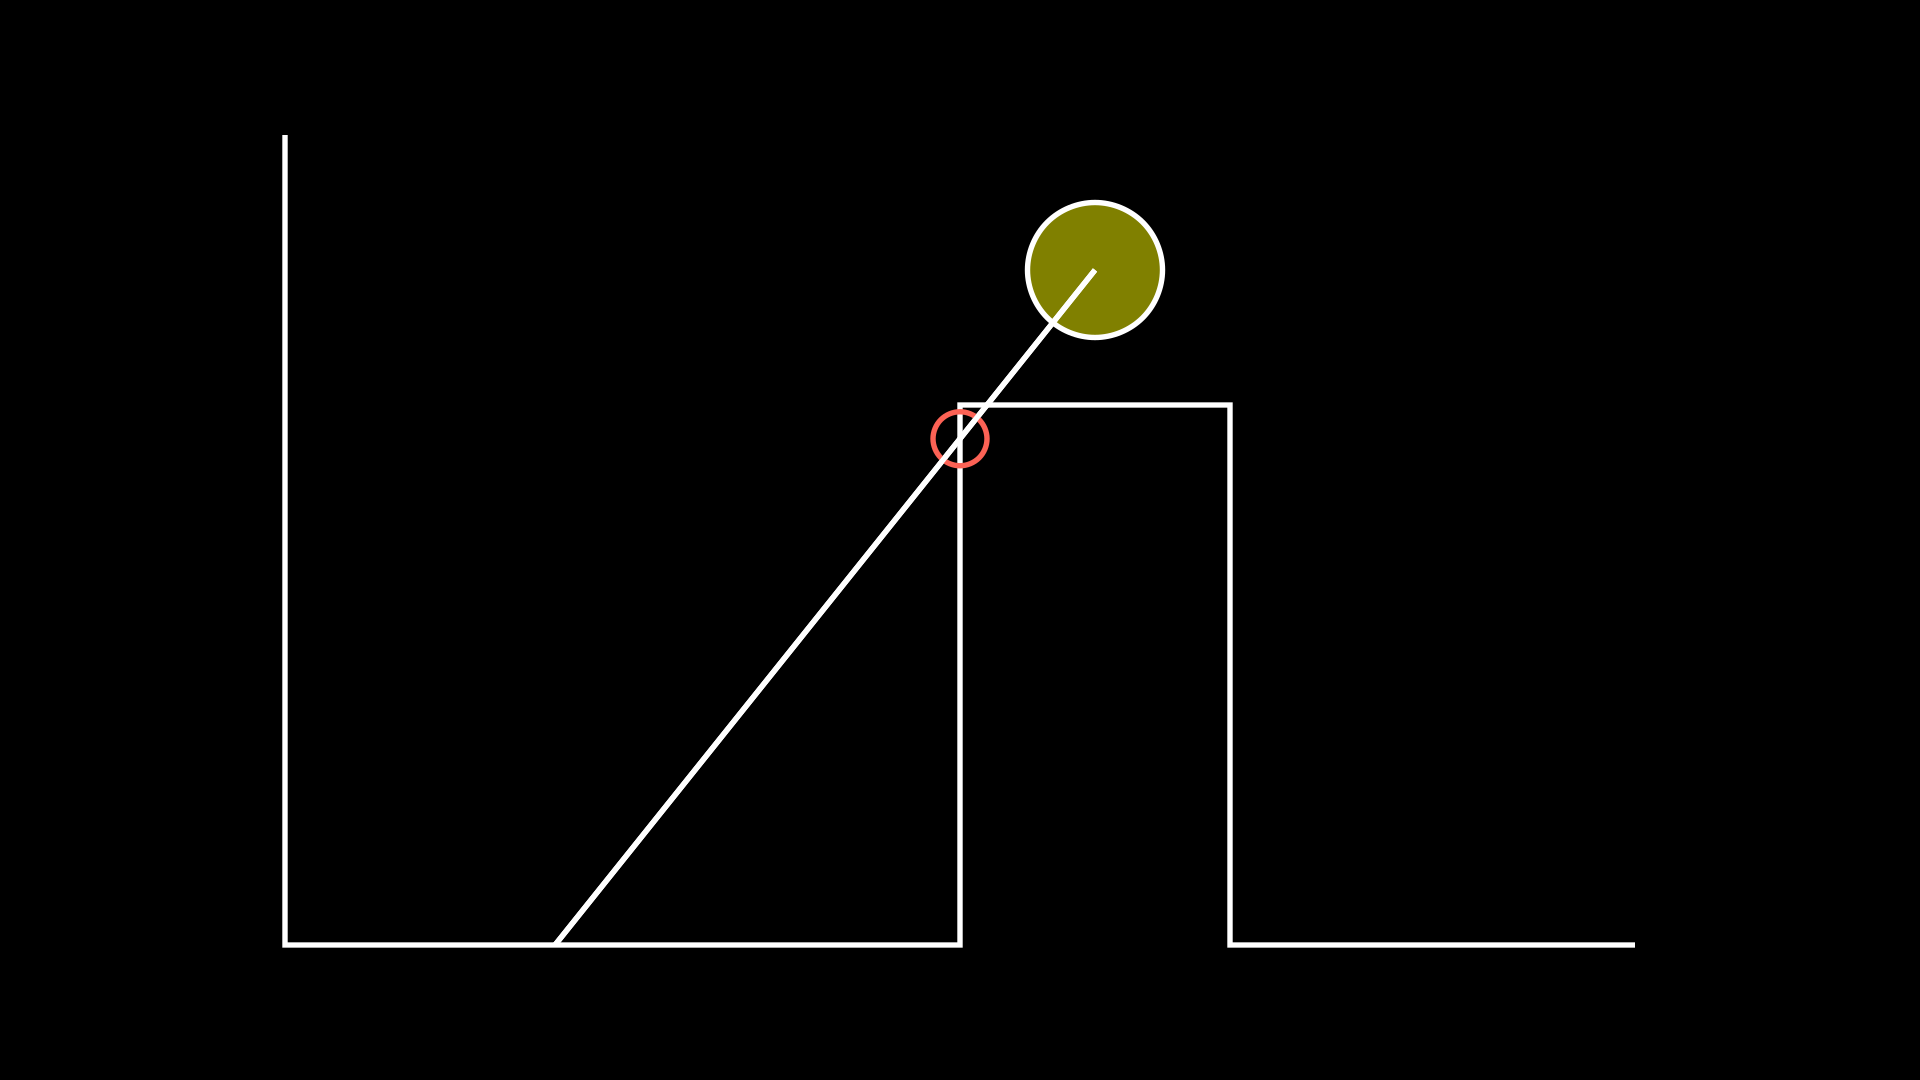
\includegraphics[width=\textwidth]{shadow-ray-diagram}
        \caption{Rayo de sombra}
    \end{subfigure}
    \begin{subfigure}{.49\textwidth}
        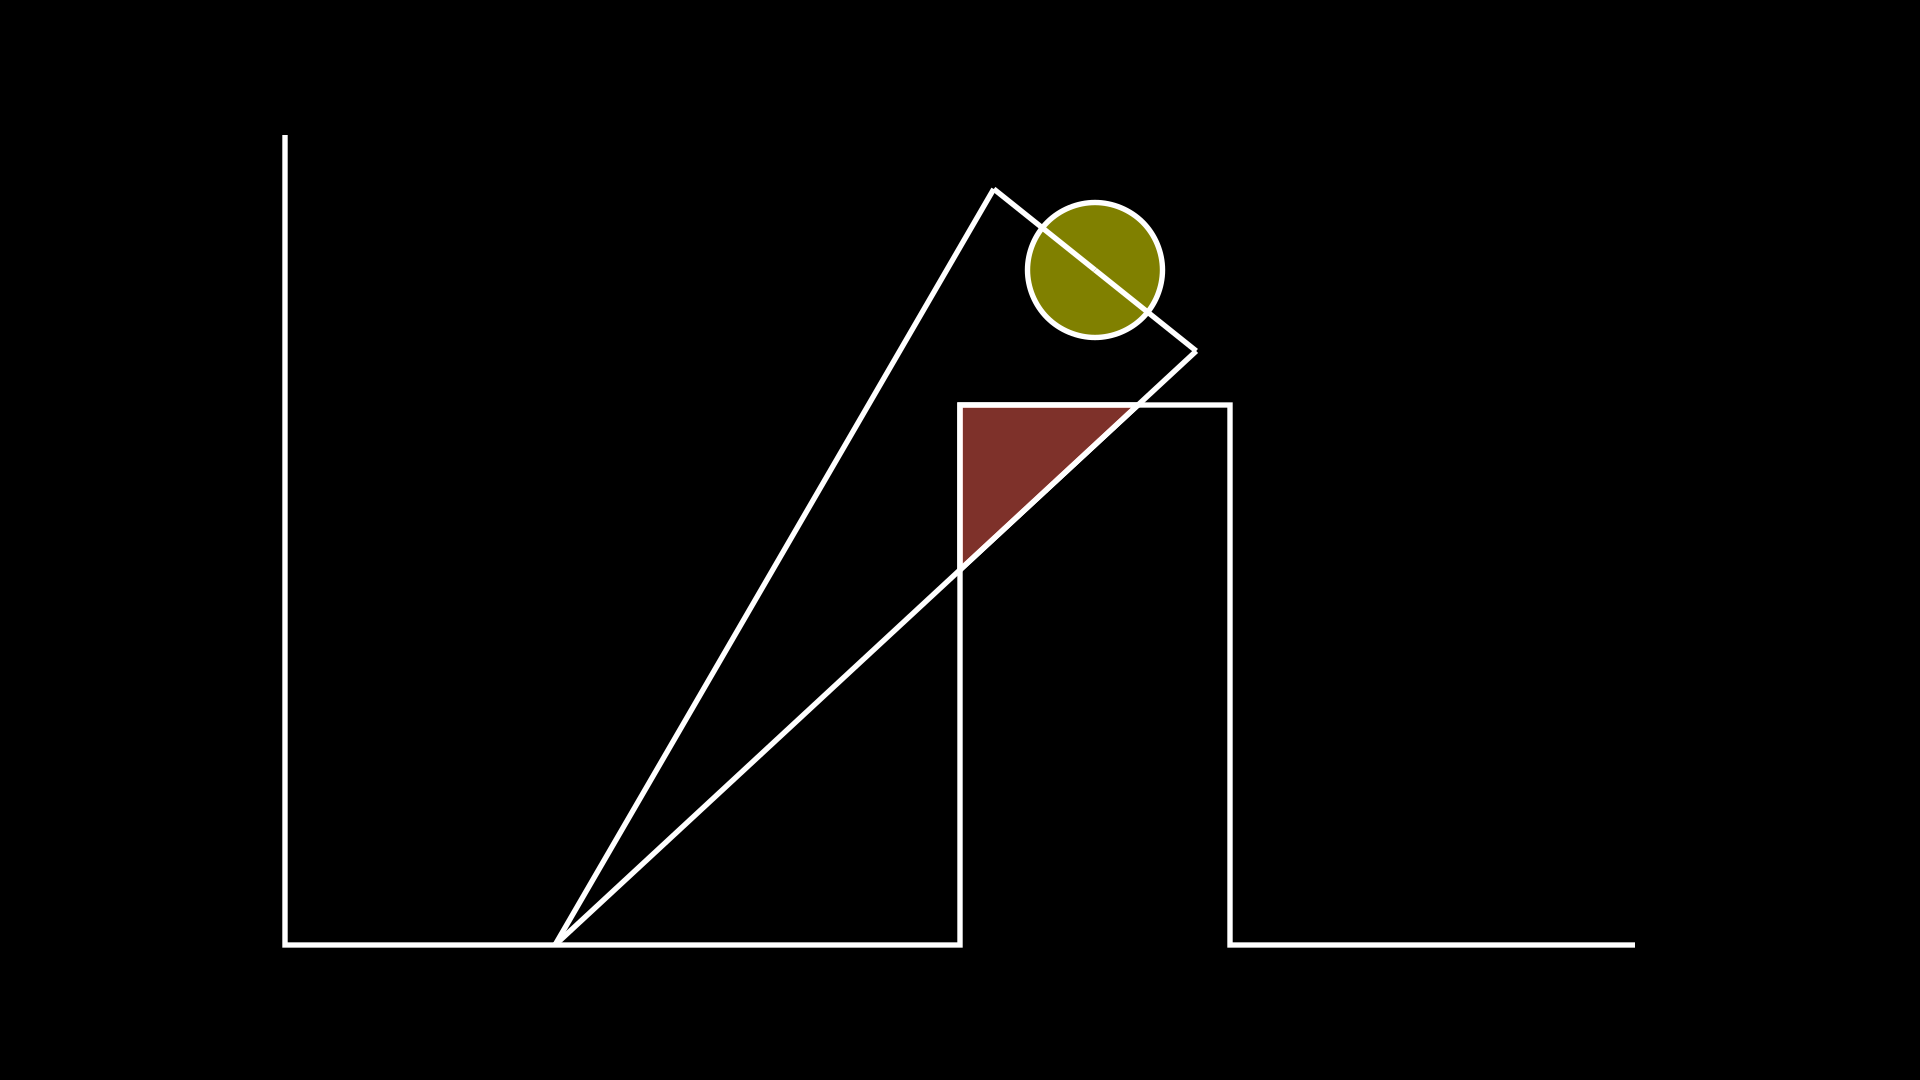
\includegraphics[width=\textwidth]{shadow-cone-diagram}
        \caption{Cono de sombra}
    \end{subfigure}
    \caption{Los conos de sombra no solo devuelven si hay intersección, también devuelven el porcentaje de área de la intersección}
    \label{fig:shadow-rays-and-cones}
    \end{center}
\end{figure}

Esta técnica sigue hallando la intersección de manera analítica, por lo que las ecuaciones son mucho más complejas.
Tanto es así que originalmente Whitted había considerado usar conos pero la complejidad añadida de las ecuaciones lo hizo descartarlos.
Aún así, los beneficios superan a las desventajas en la mayoría de los casos.

Para calcular la luz indirecta se halla la radiancia saliente de un punto en dirección a la cámara.
En \textit{path tracing}, este valor se calcula aproximando la integral sobre el hemisferio con el método de Monte Carlo.
Esto implica tomar varias muestras, que son los rayos que son lanzados desde $p$ en todas las direcciones $\omega_i$.
En el caso de trazado de conos, en lugar de rayos, se particiona el hemisferio en secciones que pueden ser aproximadas mediante estos conos, como se muestra en la figura \ref{fig:partitioned-hemisphere-cones}.

% TODO: Estaría bueno hablar del método de radiosidad antes capaz
% TODO: Se iba a llamar "Otros métodos de iluminación global" pero por ahora es uno solo jeje
\section{Photon Mapping}\label{sec:photon-mapping}

\textit{Photon Mapping}, propuesto por Henrik Wann Jensen en 2001 \cite{photon-mapping}, es un algoritmo basado en el trazado de rayos que es capaz de simular de manera más realista la refracción de la luz a través de sustancias transparentes como vidrio o agua. 
Funciona ``emitiendo'' fotones de la fuente de luz y almacenando en un mapa de fotones la ubicación de cada interacción de estos con las superficies no especulares ni transparentes de la escena.

Con \textit{photon mapping} se pueden generar cáusticas, que son los dibujos que se generan cuando una superficie especular o transparente concentra la luz en una superficie difusa.
En la figura \ref{fig:caustics} se puede ver este efecto.

% TODO: Estaría bueno poder usar imágenes generadas por nosotros en computación gráfica, pero no guardamos las imágenes en el repo como hicimos con whitted :c
\begin{figure}[h!]
    \begin{subfigure}{.5\textwidth}
        \centering
        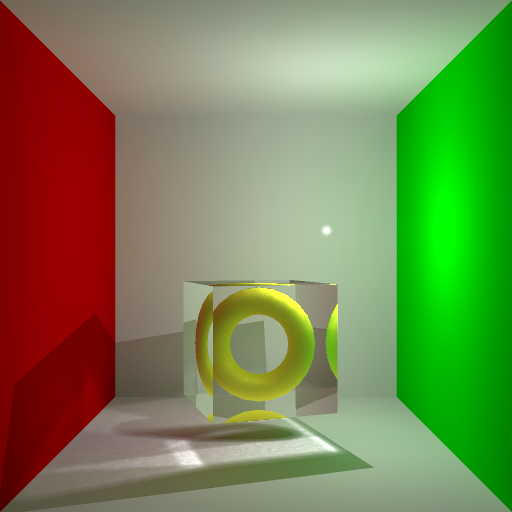
\includegraphics[width=\textwidth]{photon-mapping-cornell-box-torus.png}
        \caption{Con vidrio}
    \end{subfigure}
    \begin{subfigure}{.5\textwidth}
        \centering
        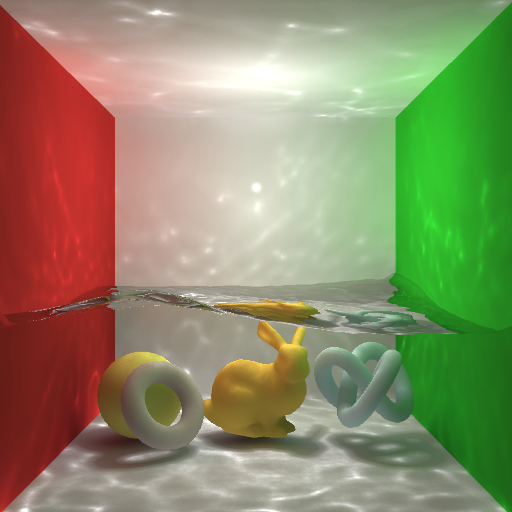
\includegraphics[width=\textwidth]{photon-mapping-cornell-box-water.png}
        \caption{Con agua}
    \end{subfigure}
    \caption{Cáusticas. Fuente: \cite{faster-photon-mapping}}
    \label{fig:caustics}
\end{figure}

El algoritmo comienza con una etapa en la que se lanzan fotones desde la fuente de luz hacia la escena.
Estos fotones se almacenan en las superficies difusas de la escena, creando un \textbf{mapa de fotones}.
Estos fotones se usan en una segundo etapa cuando se está calculando el color de un píxel.
Además de los rayos de ray tracing de reflexión y refracción, se lanzan rayos adicionales en direcciones aleatorias que buscan en el mapa de fotones, simulando la reflexión difusa.
Es una extensión a ray tracing, que utiliza el paso adicional de lanzado y evaluación de fotones.

Al igual que con el trazado de rayos, varias mejoras y optimizaciones han surgido a lo largo de los años.
Variantes de la técnica original han sido desarrolladas haciendo uso de tarjetas gráficas, alcanzando el tiempo real \cite{real-time-photon-mapping}.
Imágenes generadas por esta técnica pueden verse en la figura \ref{fig:real-time-photon-mapping}.

\begin{figure}
    \begin{subfigure}{.5\textwidth}
        \centering
        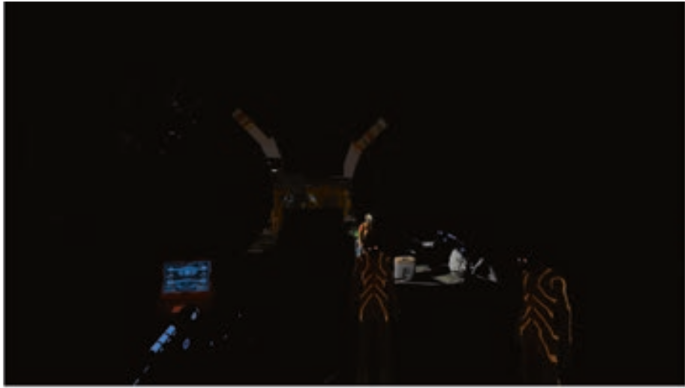
\includegraphics[width=\textwidth]{real-time-photon-mapping-direct-only.png}
        \caption{Solo luz directa}
    \end{subfigure}
    \begin{subfigure}{.5\textwidth}
        \centering
        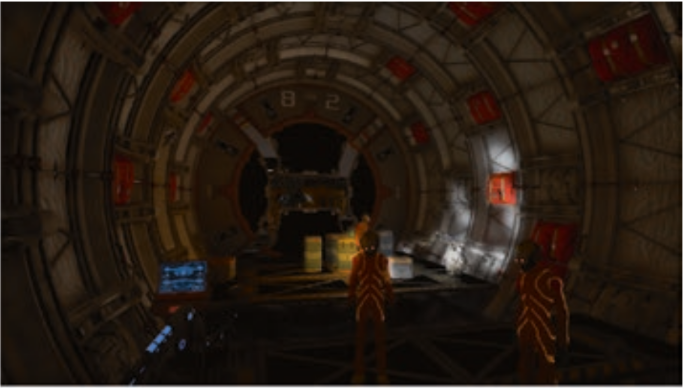
\includegraphics[width=\textwidth]{real-time-photon-mapping-indirect-only.png}
        \caption{Solo luz indirecta}
    \end{subfigure}
    \begin{subfigure}{\textwidth}
        \centering
        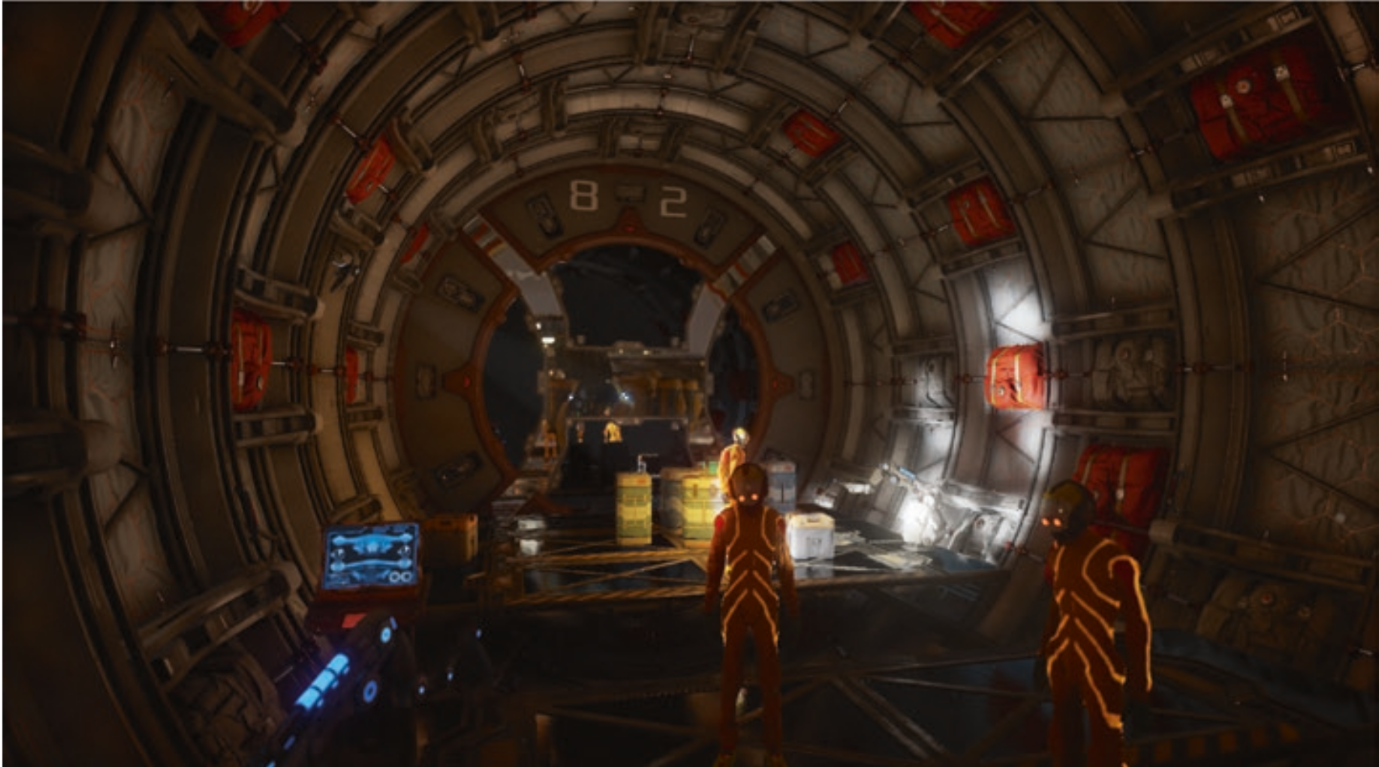
\includegraphics[width=\textwidth]{real-time-photon-mapping.png}
        \caption{Todo junto}
    \end{subfigure}
    \caption{Photon mapping en tiempo real. Fuente: \cite{real-time-photon-mapping}}
    \label{fig:real-time-photon-mapping}
\end{figure}

\section{Vóxeles}\label{sec:voxels}

Un vóxel es el equivalente de un píxel en el espacio 3D.
Así como un píxel es un elemento de imagen, \textit{\textbf{pi}cture \textbf{el}ement}, un vóxel es un elemento de volumen, \textit{\textbf{vo}lume \textbf{el}ement} \cite{rtr}.
Similar a como los píxeles se ubican en una grilla que divide una superficie 2D en secciones cuadradas, los vóxeles dividen un volumen 3D en cubos.

Tradicionalmente, se usan para guardar datos volumétricos y como primitiva para renderizar una variedad de objetos.
Permiten representar volúmenes, en contraposición al triángulo, que se utiliza para representar únicamente superficies.
Son un buen candidato para renderizar volúmenes y modelos 3D como el humo, la niebla, el fuego, los huesos y el terreno, entre otros.

Algunos de estos elementos se ven en la figura \ref{fig:voxels_for_rendering}. % TODO: Encontrar fotos más nuevas, estas se ven que son viejasas

\begin{figure}
    \begin{center}
        \begin{subfigure}{.49\textwidth}
            \centering
            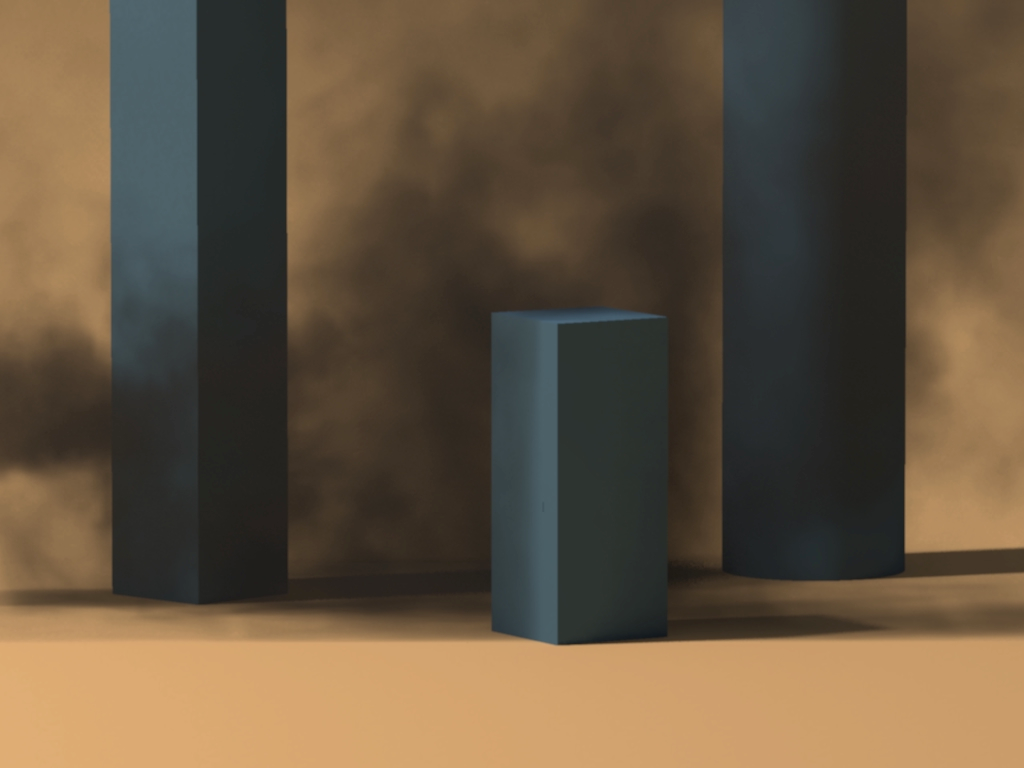
\includegraphics[width=\textwidth]{voxel-smoke.png}
            \caption{Vóxeles representando humo. Fuente: \cite{voxel-smoke}}
        \end{subfigure}
        \begin{subfigure}{.49\textwidth}
            \centering
            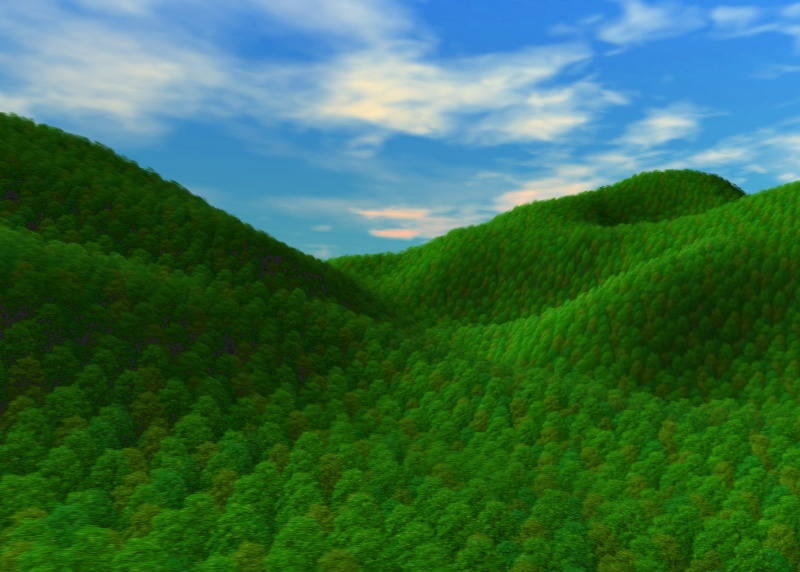
\includegraphics[width=\textwidth]{voxels-for-trees.png}
            \caption{Vóxeles representando vegetación. Fuente: \cite{voxels-for-trees}}
        \end{subfigure}
    \end{center}
    \caption{Vóxeles para renderizar humo y vegetación}
    \label{fig:voxels_for_rendering}
\end{figure}

% TODO: Completar con papers
% Los vóxeles también son utilizados para visualizaciones científicas.

% Además de primitiva de renderizado, los vóxeles se utilizan cada vez más para manipular datos espaciales, como en NST (\textit{Neural Style Transfer}) \cite{transport-based-neural-style-transfer}, que fue utilizado en la reciente película de Pixar \textit{Elemental} \cite{elemental-neural-style-transfer}.

Cada vóxel marca si la zona del espacio que representa está ocupada o libre, y por ejemplo en contextos médicos se usan para indicar la opacidad y densidad de un hueso.
Para el renderizado, se pueden utilizar para almacenar valores como el color o la irradiancia en cada vóxel.
En general, no es necesario guardar la posición de un vóxel, ya que su lugar en la grilla es lo que indica su posición.

El proceso de convertir otra representación, por ejemplo una malla de polígonos, en una estructura de vóxeles se llama voxelización.
Esto involucra intersecar la representación con la grilla de vóxeles, y marcar como ocupados los vóxeles que se solapen con esta.

Algunos programas usan grillas completas de vóxeles.
Sin embargo, en la mayoría de los casos no es necesario.
Una observación útil es que en muchas aplicaciones es suficiente tener vóxeles en el límite entre un objeto y el espacio vacío, siendo innecesario el relleno.

Otra observación útil es que, para una buena representación, es suficiente con tener mucho detalle en la frontera entre espacio vacío y lleno.
Para lograr esto, se puede usar un \textit{octree} disperso, que será explicado a continuación.

\section{Octrees}\label{sec:octree}

Un \textit{octree} es una estructura de datos de ``árbol'', en la que cada nodo interno (no hoja) tiene $8$ hijos \cite{rtr}.
Suele usarse para representar datos espaciales \cite{octree-textures}.
Se puede utilizar para dividir el espacio 3D de manera jerárquica, con varios niveles.

Se parte de un volumen original cúbico o paralelepípedo que se divide en dos partes iguales por dimensión, resultando en $8$ octantes iguales.
En la estructura de árbol, el nodo raíz representa el volumen original y cada uno de sus $8$ hijos representa a cada octante.
Aplicando recursivamente, se divide el espacio en $8^{(n - 1)}$ secciones, donde $n$ es la cantidad de niveles del árbol, y el primer nivel tiene un solo nodo que representa toda la escena.

De manera similar, un espacio 2D se puede dividir utilizando un \textit{quadtree}, en donde cada nodo interno tiene $4$ hijos.
Los \textit{quadtrees}, al ser bidimensionales, son más fáciles de visualizar, por lo que serán utilizados a lo largo de este informe para explicar aspectos que funcionan igual tanto en ellos como en su equivalente tridimensional.
En la figura \ref{fig:quadtree} se muestra un \textit{quadtree} en su forma de árbol y en el espacio que subdivide.

\begin{figure}
    \begin{subfigure}{\textwidth}
        \centering
        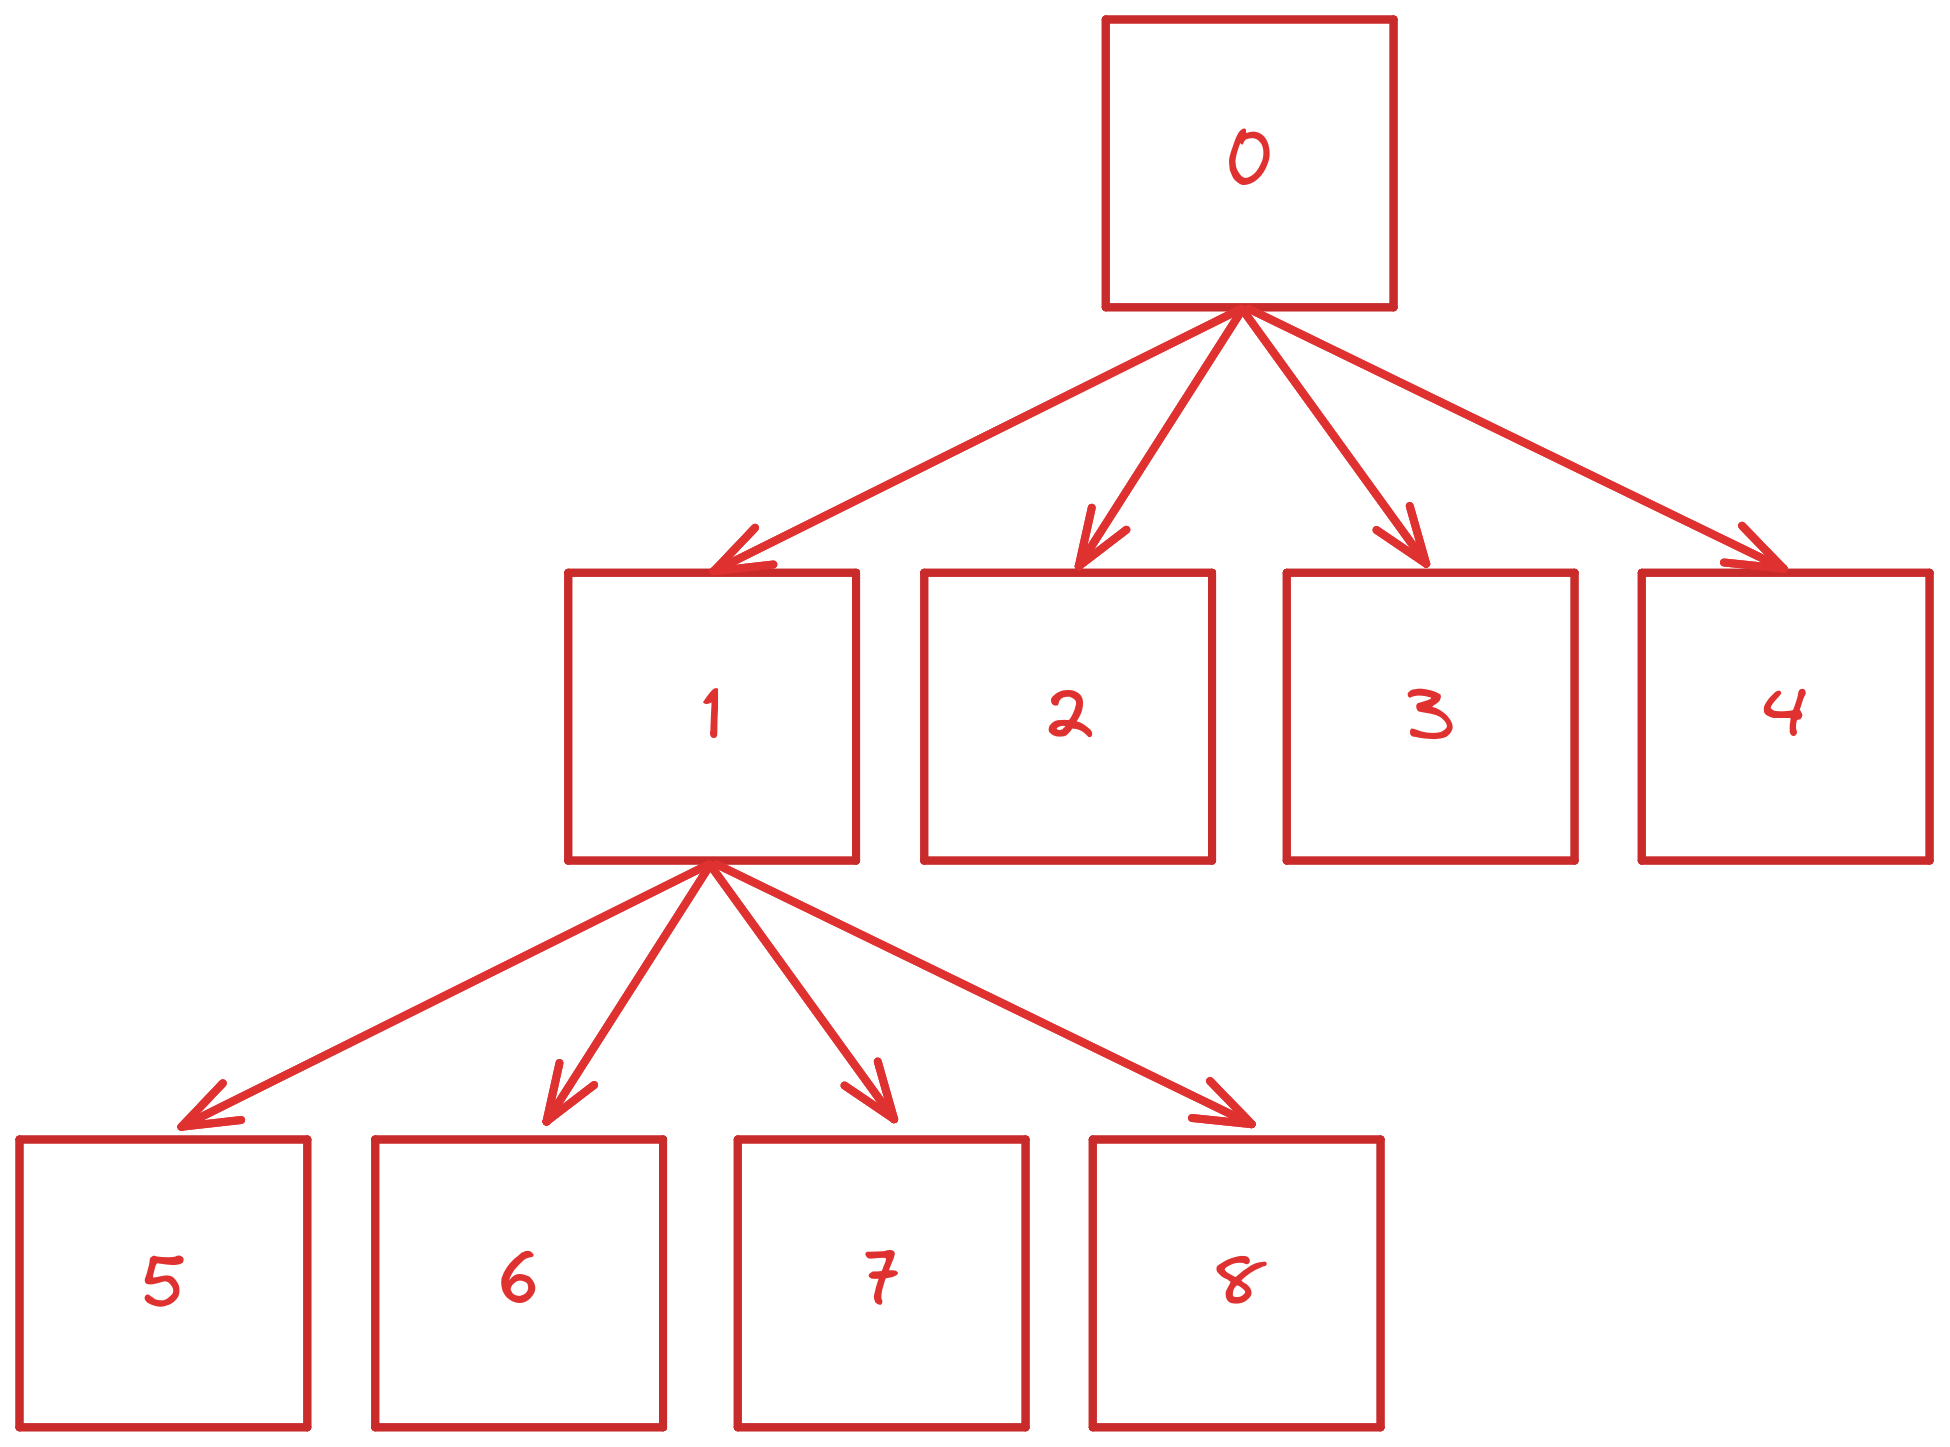
\includegraphics[width=.4\textwidth]{quadtree.png}
        \caption{Visto en su estructura de árbol, con punteros a cada hijo}
    \end{subfigure}
    \begin{subfigure}{\textwidth}
        \centering
        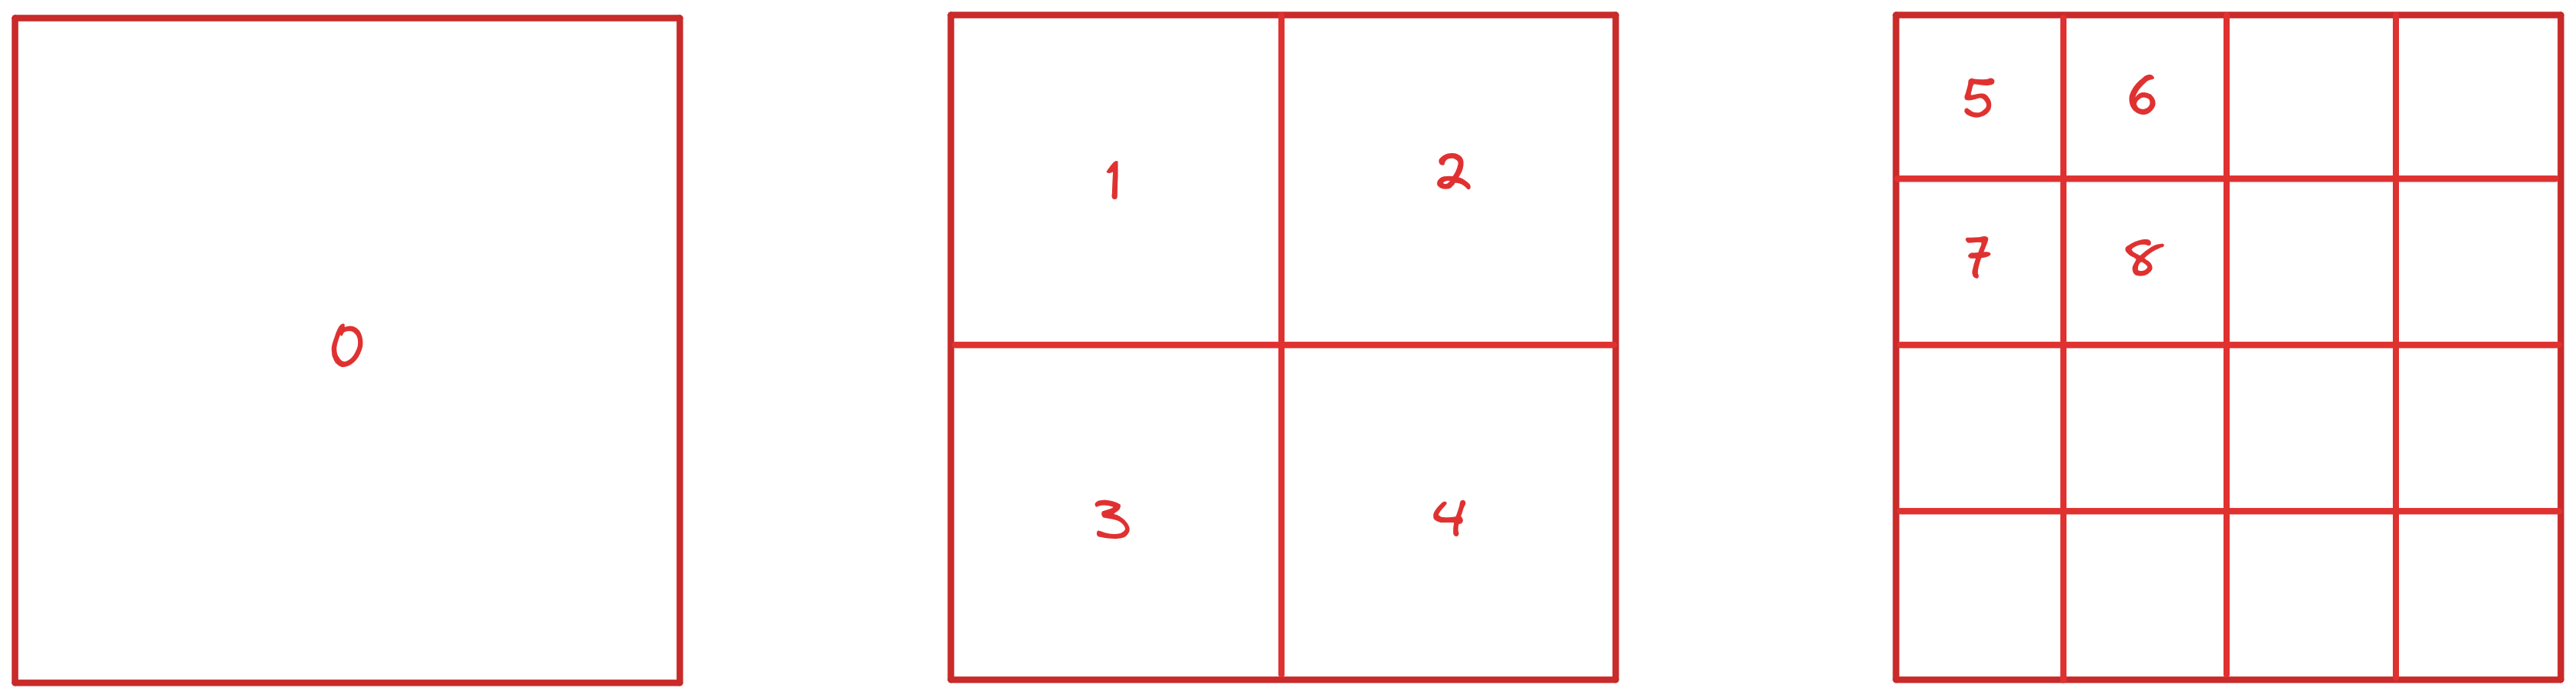
\includegraphics[width=.6\textwidth]{quadtree-spatial.png}
    \caption{Visto espacialmente}
    \end{subfigure}
    \caption{Quadtree}
    \label{fig:quadtree}
\end{figure}

Cuando la naturaleza de la información lo permite, se puede evitar subdividir un nodo del árbol si sus $8$ hijos tienen todos la misma información.
De esta idea surge el \textit{octree} disperso.

A la hora de voxelizar una escena, los vóxeles pueden ubicarse dentro de un \textit{octree} disperso, en lugar de en una grilla.
En este caso, los nodos no se subdividen si no hay geometría dentro de la región del espacio que representan, dado que no hay vóxeles en esa región.

% TODO: Imagen de esto

\section{Ducto gráfico}\label{sec:graphics-pipeline}

Dada una escena 3D, una cámara virtual, varios objetos y varias fuentes de luz, ¿cómo se genera una imagen 2D en el monitor de una computadora?

Si bien es posible generar una imagen a partir de una escena usando la CPU, las GPUs, o tarjetas gráficas, están especialmente diseñadas para esto.

Las tarjetas gráficas ejecutan un \textbf{ducto gráfico} para generar las imágenes.
Esto es, una secuencia de transformaciones y operaciones que parten de primitivas y generan la imagen final.
Existen varios tipos de ductos gráficos, el ducto raster, el de cómputo de propósito general, el de trazado de rayos, entre otros.
El ducto raster es importante, dado que es utilizado en \textit{voxel cone tracing}.

El ducto raster parte de vértices de mallas poligonales, aplica transformaciones, realiza pruebas de profundidad y calcula el color de cada píxel de la imagen final.

Cada paso de un ducto gráfico puede ser fijo o programable.
En el caso de que sea fijo, el mismo ya está implementado en la tarjeta gráfica.
En algunos casos, estos pasos fijos proveen parámetros para configurar su comportamiento, este es su mayor grado de libertad.
En el caso de que sea programable, se puede escribir un \textit{shader}, un programa de sombreado que corre en la GPU, que implementa el paso en su totalidad.
Esto aporta un gran grado de libertad a la hora de renderizar escenas.

Existen varias APIs, interfaces, con las que se puede interactuar con una tarjeta gráfica \cite{comparison-graphics-apis}, notablemente Vulkan, Direct3D, Metal, WebGPU y OpenGL.
Todas estas permiten acceder al ducto de raster.

En OpenGL, por ejemplo, este ducto posee las etapas que se ven en la figura \ref{fig:raster-pipeline} \cite{rtr}.

\begin{figure}[h!]
    \centering
    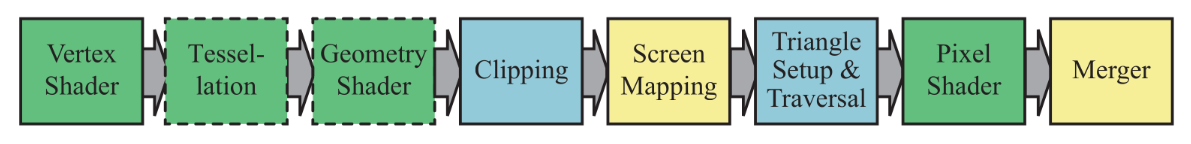
\includegraphics[width=\textwidth]{raster-pipeline.png}
    \caption{Ducto de raster. Fuente: \cite{rtr}}
    \label{fig:raster-pipeline}
\end{figure}

De estas, tres son programables.
El desarrollador debe escribir \textit{shaders} para estos pasos, que se pueden escribir en el lenguaje GLSL \cite{glsl-spec}.
Los \textit{shaders} son programas que ejecutan en la GPU.
Estos programas son ejecutados con un alto grado de paralelización en la tarjeta gráfica.

Las etapas programables son el \textit{vertex shader} (\textit{shader} de vértices), \textit{geometry shader} (geometría), y \textit{fragment} o \textit{pixel shader} (fragmentos o píxeles).
Cada una de estas etapas pueden comunicar datos a etapas posteriores.
El resto de las etapas son fijas.

El \textit{vertex shader} toma los vértices de la geometría de la escena y los puede transformar a otro sistema de coordenadas.
En general es usado para pasar los vértices de espacio local de coordenadas a espacio global, de vista y luego proyección.
Esto se logra usando tres matrices que se conocen como modelo, vista y proyección.
Un hilo es ejecutado por cada vértice de las primitivas de entrada.

El \textit{geometry shader} puede generar nuevos vértices, por lo que es útil para agregar complejidad extra a la geometría de la escena.
Aquí se ejecuta un hilo por cada primitiva de salida del \textit{vertex shader}, pero estas primitivas pueden tener más de un vértice.

Finalmente, el \textit{fragment shader} (o \textit{pixel shader}) trabaja con píxeles y no con vértices.
Es en este \textit{shader} donde se realizan los cálculos de iluminación para calcular el color de cada píxel.
Se ejecutan mínimo un hilo por cada píxel de la imagen que se quiere generar.
Pueden ejecutarse más de uno en el caso que dos objetos aporten color al mismo píxel, en cuyo caso puede ser que uno sea descartado o pueden mezclarse los colores de ambos en caso de que sean transparentes.

Otro ducto muy relevante, que es usado para implementar la mayoría del algoritmo, es el ducto de cómputo de propósito general.
Este es muy simple, consiste en la inicialización de datos de entrada, luego la ejecución de un programa en la GPU llamado \textit{compute shader} (\textit{shader} de cómputo) y finalmente el retorno de datos hacia la CPU.
Notar que este ducto no es utilizado para generar una imagen, sino para realizar cálculos arbitrarios que toman una entrada y producen una salida, aprovechando la alta paralelización que provee la tarjeta gráfica.

% TODO: Agregar una referencia acá
\section{Renderizado diferido}\label{sec:deferred-rendering}

A la hora de renderizar una escena, hay dos grandes modelos que se pueden utilizar: el clásico, conocido como \textit{forward rendering} y una opción alternativa conocida como renderizado diferido.

En el primero, se procesan todos los vértices en el programa.
Cada uno pasa por cada etapa del ducto gráfico y aporta a la imagen final a menos que sea desechado por un test de profundidad.
Cuando un pixel genera varios fragmentos, y se deben correr calculos pesados por fragmento, se puede estar realizando trabajo innecesario. Esto ocurre porque si se hace un test de profundidad solo uno de los fragmentos va a ser necesario para darle valor fianl al pixel, mientas el resto va a ser descartado.

En el renderizado diferido, se procesan todos los vértices del programa pero se saltean calculos pesados en el \textit{fragment shader}.
Se guarda toda la información necesaria para etapas posteriores en texturas llamadas \textit{geometry buffers}, datos como posicion, normal, color y cualquier otro dato relevante de la geometria a la hora se realizar calculos pesados de sombreado.
Al hacer esto, se ahorran los cálculos para todos las geometrias que son desechadas, al estar fueras de vista pero igual generar fragmentos que utilizan computo en el \textit{fragment shader}, reduciendo lo calculos pesados solo para partes de la escena que van a aparecer en pantalla. % TODO: Es durante o después
% TODO: Hablar del volumen de vista?
Estos suelen ser un buen porcentaje del total, teniendo en cuenta los objetos fuera del ángulo de vista y detrás de otros objetos.

El \textit{forward rendering} es conceptualmente más sencillo y más fácil de implementar.
En escenas con pocos objetos y fuentes de luz, o con calculos simples de iluminacion, la complejidad extra del renderizado diferido no está justificada dado que el aumento de rendimiento es despreciable.
A su vez, \textit{forward rendering} soporta mejor la transparencia.
Sin embargo, a medida que la complejidad de la escena y los metodos de sombreado aumenta, el renderizado diferido se vuelve cada vez una mejor opción para aumetentar el rendimiento.
También, el renderizado diferido facilita ciertas técnicas de post-procesamiento de la imagen, como bloom, HDR (High Dynamic Range), corrección gamma, y normalización, entre otras.

% \section{Integral de rendering}

% Ya fue mencionada la ecuación de rendering \ref{eq:rendering-equation}.
% % TODO: Esto es teoría de la luz en general, ver cómo ponerlo
% Este modelo se basa en la óptica geométrica, que asume que la luz se propaga en una linea recta cuando no tiene interacción con la materia, en contraste con la óptica física, que considera la característica de onda de la luz y sus dos posibles estados de polarización.

% La energía de luz se describe por su radiancia $I(x, \omega)$.
% Describe el campo de radiación en un punto $x$, dada la dirección $\omega$.
% Se expresa en $W\cdot sr^{-1}\cdot m^{-2}$ y se define como:

% \begin{equation}
%     I(x, \omega) = \frac{dQ}{dA\cdot cos\theta\cdot d\Omega\cdot dt}
% \end{equation}

% con $Q$ la energía radiante (en Joules), $A$ el área (en $m^2$), $\theta$ el ángulo entre la dirección de la luz $\omega$ y el vector normal a la superficie, y $\Omega$ el ángulo sólido (en estereorradianes).

% La radiancia a lo largo de un rayo de luz es afectada cuando pasa por un medio participativo.
% Esta interacción entre la luz y la materia se modela con tres tipos de interacciones: emisión, absorción y dispersión.

% Emisión describe la cantidad de energía radiante de luz que se emite directamente por el medio participativo.
% Absorción es la cantidad de energía que es absorbida por el material.
% Finalmente, la dispersión describe la cantidad de energía que es dispersada por el material, cambiando la dirección de la propagación de la luz.
% La dispersión puede tanto incrementar (dispersión entrante) como reducir (dispersión saliente) la energía a lo largo del rayo.

% La ecuación de la transferencia de luz se obtiene combinando estos tres efectos:

% \begin{equation}
%     \omega \cdot \nabla_x I(x, \omega) = -\chi I(x, \omega) + \eta
% \end{equation}

% donde $\nabla_x I$ es la derivada direccional (el gradiente) de la radiancia.
% El producto escalar entre la dirección de la luz $\omega$ y el gradiente de la radiancia $\nabla_x I$ describe el gradiente tomado en la dirección de la luz.
% El término $\chi(x, \omega)$ es el coeficiente de absorción total.
% Se define como la suma de $\kappa(x, \omega)$, el verdadero coeficiente de absorción, y $\sigma(x, \omega)$, el coeficiente de dispersión saliente:

% \begin{equation}
%     \chi = \kappa + \sigma
% \end{equation}

% La razón $\frac{\sigma}{\chi}$ de coeficiente de dispersión saliente sobre coeficiente de dispersión total es el \textit{albedo}.
% Un albedo de $1$ significa que no hay absorción, hay dispersión perfecta.

% El término $\eta(x, \omega)$ de la ecuación es el coeficiente de emisión total.
% Es la suma del coeficiente de emisión real $q(x, \omega)$ y el coeficiente de dispersión entrante $j(x, \omega)$:

% \begin{equation}
%     \eta = q + j
% \end{equation}

% Mientras $\kappa$, $\sigma$ y $q$ son propiedades ópticas del material, el coeficiente de dispersión entrante $j$ tiene que ser calculado integrando la contribución de todas las direcciones entrantes de luz sobre la esfera:

% \begin{equation}
%     j(x, \omega) = \frac{1}{4\pi} \int_\Omega \sigma(x, \omega')\cdot p(x, \omega', \omega'')\cdot I(x, \omega')\cdot d\omega'
% \end{equation}

% Las contribuciones de la luz incidente $I(x, \omega')$ son pesadas por tanto el coeficiente de dispersión $q$ y una \textit{función de fase} $p(x, \omega', \omega)$ que describe la probabilidad de dispersión desde la dirección entrante $\omega'$ hacia la dirección $\omega$.

% Como usualmente consideramos la transferencia de luz a través de un solo rayo, podemos reescribir la ecuación para considerar un parametro $s$ a lo largo del rayo expresado como $x = p + s\omega$, con $p$ un punto de referencia arbitrario en el rayo:

% \begin{equation}\label{eq:light_transfer}
%     \frac{dI(s)}{ds} = -\chi(s)I(s) + \eta(s)
% \end{equation}

% En vóxel cone tracing, se usa el modelo óptico de emisión-absorción, descrito en \cite{real-time-volume-graphics}.
% En este modelo, se ignora la dispersión y la iluminación indirecta, representando solo emisión y absorción.
% La ecuación \ref{eq:light_transfer} queda:

% \begin{equation}
%     \frac{dI(s)}{ds} = -\kappa(s)I(s) + q(s)
% \end{equation}

% Esta ecuación se puede resolver transformandola en una integral pura entre un punto de comienzo en el rayo $s = s_0$ y un punto de fin $s = D$.
% Definimos $I_0$ como la radiancia inicial.
% La integral resultante es:

% \begin{equation}
%     I(D) = I_0\cdot e^{-\tau(s_0, D)} + \int_{s_0}^D q(s)\cdot e^{-\tau(s, D)}\cdot ds
% \end{equation}

% El término $\tau(s1, s2)$ se llama la profundidad óptica o grosor óptico.

% % TODO: Estaría bueno hablar de todas las referencias que habla el paper acá sobre luz. Completar.
% % Hay hasta un par de papers que usan vóxels, solo un poco distinto a ellos.
% % Cuando arrancó la tésis, tendríamos que habernos mandado de una a leer todas estas referencias.
% Las mejores soluciones en terminos de velocidad trabajan en el espacio de imágen en lugar del espacio del mundo.
% vóxel cone tracing es menos eficiente que esas soluciones pero no requiere aproximaciones tan fuertes.

% % TODO: Volver a poner la parte de normlaes si realmente usamos normales.
% % Ojalá no.

% % \section{Filtrado de normales}\label{sec:normal_filtering}

% % Filtrar datos geométricos, como las normales, no es tan fácil como con colores.
% % El problema, como se muestra en la figura \ref{fig:ndf}, es que dos normales en direcciones opuestas, al ser promediadas, no representan correctamente la región conjunta.
% % Todos los enfoques para filtrar normales se basan en la idea de representar la información de las normales como una distribución estadística de direcciones.
% % Esta representación se define por una función de distribución de normales (NDF, por sus siglas en inglés), que dada una dirección, devuelve la densidad de normales para cada punto de la superficie.

% % \begin{figure}[h!]
% %     \centering
% %     \includegraphics[width=\textwidth]{figs/ndf.png}
% %     \caption{El problema filtrando normales. Fuente: \cite{normal-map-filtering}}
% %     \label{fig:ndf}
% % \end{figure}

% % \cite{toksvig} propuso una representación muy compacta para un NDF.
% % Esta representación se basa en solo una dirección media no normalizada generalmente computada con un mipmap simple de un normal map.
% % El largo de este vector media se usa como una medida de la consistencia de las direcciones normales de la superficie, y se usa para estimar la desviación estándar de una distribución Gaussiana.


% diseño
\graphicspath{{chapters/5_experimentos/figures/}}

\chapter{Experimentación}\label{chap:experiments}

Para analizar el rendimiento de la implementación, se realizaron experimentos en distintas tarjetas gráficas, las cuales se ven en el Cuadro \ref{tab:hardware-used}.
Estas, $H1$, $H2$ y $H3$, corresponden a hardware con capacidades gráficas progresivamente superiores.
Las escenas utilizadas se muestran en las figuras \ref{fig:cornell-box-full} y \ref{fig:sponza}, que llamaremos $S1$ y $S2$ respectivamente.
Se puede observar en cada una de ellas la luz indirecta difusa, luz indirecta especular y sombras suaves.

\begin{table}[ht]
	\centering
	\begin{tabular}{|c|c|c|c|c|}
		\hline
		\textbf{Nombre} & \textbf{GPU} & \textbf{Núcleos} & \textbf{Clock (GHz)} & \textbf{VRAM (GB)} \\
		\hline
		$H1$ & Intel Mesa ADL GT2 & 96 & 1.45 & * \\
		\hline
		$H2$ & Nvidia GTX 1660 Ti mobile & 1536 & 1.45 & 6 \\
		\hline
		$H3$ & Nvidia Geforce RTX 4070 & 5888 & 1.92 & 12 \\
		\hline
	\end{tabular}
	\caption{Hardware utilizado. * al ser una tarjeta integrada, no tiene memoria gráfica dedicada.}
	\label{tab:hardware-used}
\end{table}

\begin{figure}[H]
	\centering
	  \begin{subfigure}{0.49\textwidth}
	      \centering
	  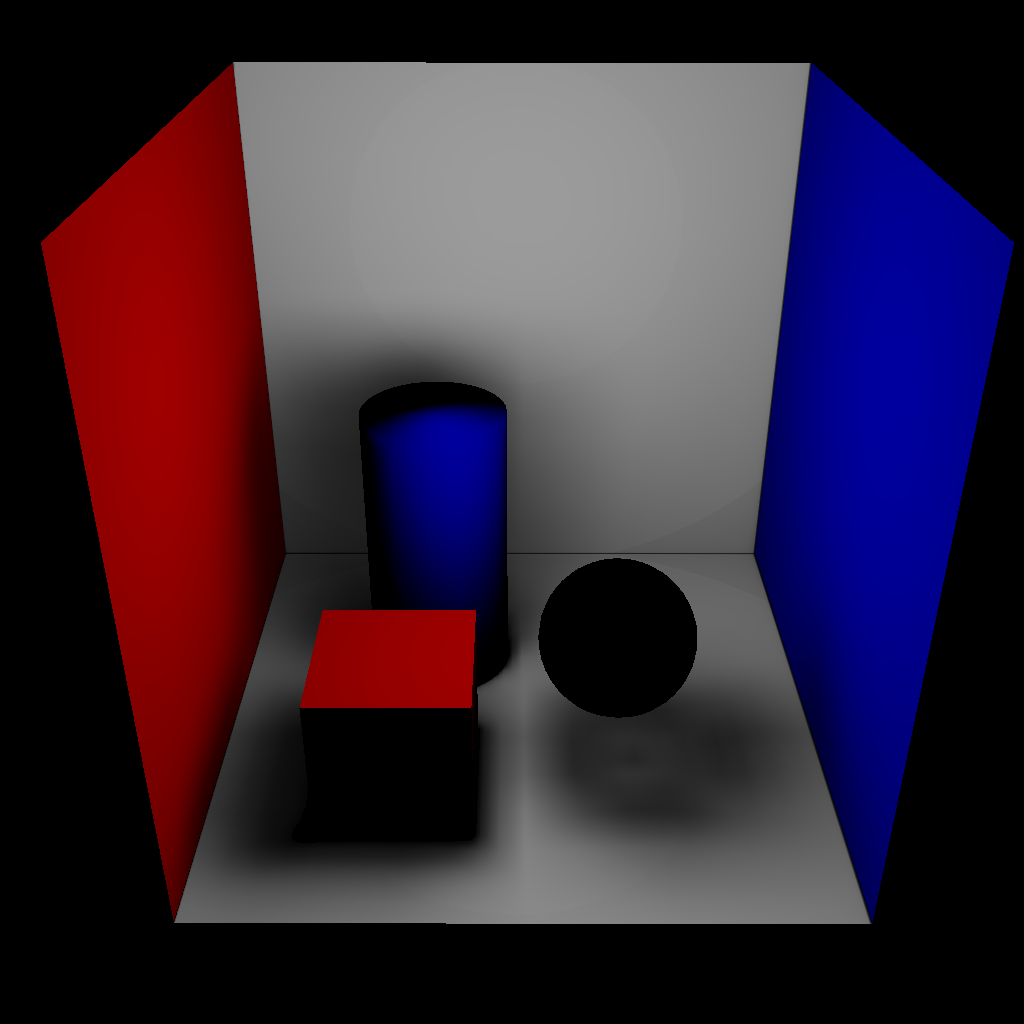
\includegraphics[width=\textwidth]{cornell-box-direct.png}
	      \caption{Solo luz directa.}
	  \end{subfigure}
	  \begin{subfigure}{0.49\textwidth}
	      \centering
	  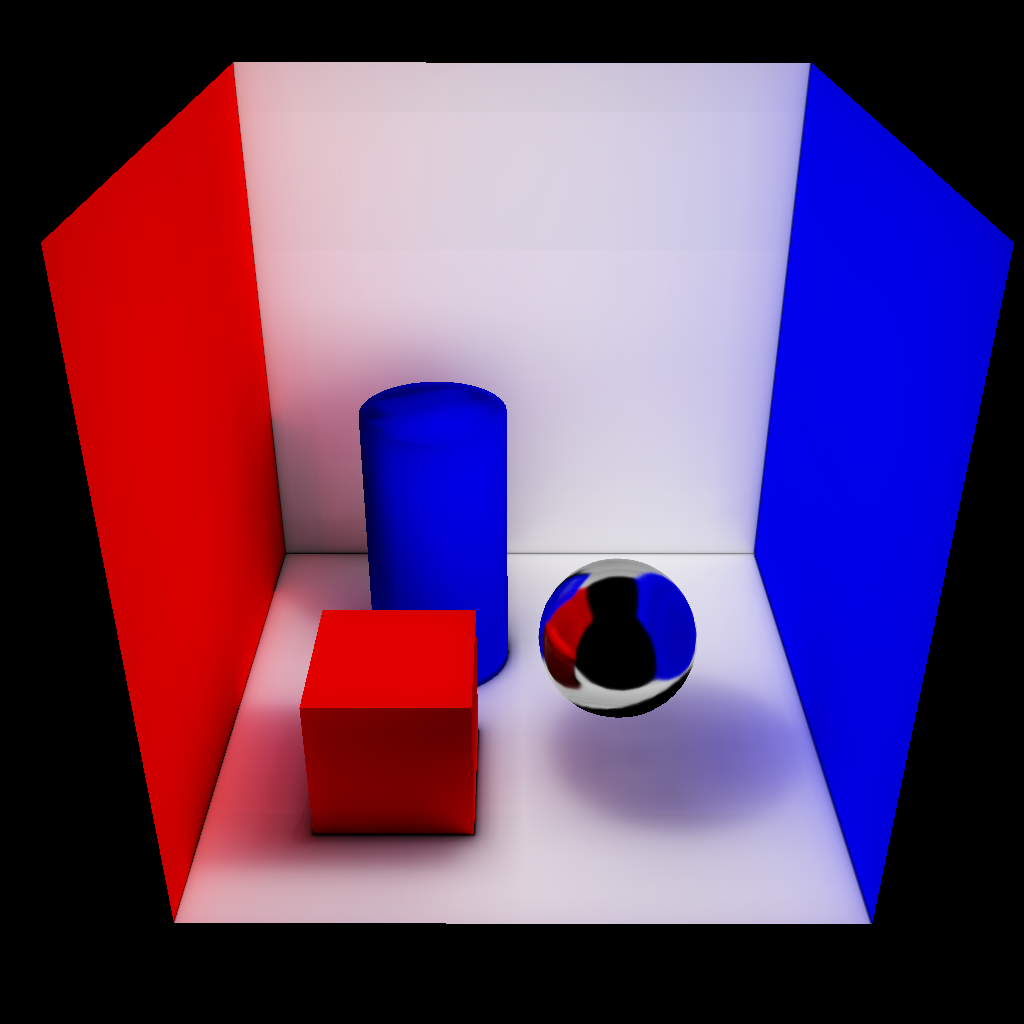
\includegraphics[width=\textwidth]{cornell-box-full.png}
	      \caption{Luz directa e indirecta.}
	  \end{subfigure}
	\caption{Escena de prueba con geometría simple.}
	\label{fig:cornell-box-full}
\end{figure}

\begin{figure}[H]
	\begin{subfigure}{0.49\textwidth}
	  \centering
	  \includegraphics[width=\textwidth]{sponza-direct.png}
	  \caption{Solo luz directa.}
	\end{subfigure}
	\begin{subfigure}{0.49\textwidth}
	  \centering
	  \includegraphics[width=\textwidth]{sponza-all.png}
	  \caption{Luz directa e indirecta.}
	\end{subfigure}
	\caption{Sponza.}
	\label{fig:sponza}
\end{figure}

Los experimentos varían la cantidad de vóxeles por dimensión, y registran los cuadros por segundo alcanzados (FPS, por sus siglas en inglés) y el tiempo de construcción del \textit{octree} en segundos.
Para conseguir los FPS se ejecutó el programa durante un minuto, tomando una muestra cada segundo, luego se promediaron.
Para el tiempo de construcción del \textit{octree}, se construyó 50 veces y se calculó el tiempo promedio.
Cada ejecución se realizó independientemente, para evitar posibles mejoras debido al uso del caché.

En el Cuadro \ref{tab:experiment-results} se muestran los resultados de estos experimentos en los 3 hardwares utilizados ($H1$, $H2$ y $H3$) descritos en el Cuadro \ref{tab:hardware-used}.
Se muestran los resultados para cada una de las escenas $S1$ y $S2$, en cada uno de los hardwares, y para cada nivel de resolución (vóxeles por dimensión).

\begin{table}[ht]
\centering
\begin{tabular}{|c|c|c|c|c|}
	\hline
	\textbf{Escena} & \textbf{Hardware} & \textbf{Vóxeles} & \textbf{FPS} & \textbf{Construcción del \textit{octree} (s)} \\
	\hline
	$S1$ & $H1$ & $256$ & $18.22$ & $1.76$ \\
	\cline{3-5}
	 & & $512$ & $14.77$ & $1.82$ \\
	\cline{3-5}
	 & & $1024$ & $12.13$ & $2.01$ \\
	\cline{2-5}
	 & $H2$ & $256$ & $136.57$ & $1.78$ \\
	\cline{3-5}
	 & & $512$ & $108.67$ & $1.80$ \\
	\cline{3-5}
	 & & $1024$ & $60.24$ & $1.89$ \\
	\cline{2-5}
	 & $H3$ & $256$ & $141.57$ & $1.88$ \\
	\cline{3-5}
	 & & $512$ & $141.47$ & $1.90$ \\
	\cline{3-5}
	 & & $1024$ & $140.88$ & $1.89$ \\
	\hline
	$S2$ & $H1$ & $256$ & $7.30$ & $1.84$ \\
	\cline{3-5}
	 & & $512$ & $4.29$ & $1.86$ \\
	\cline{3-5}
	 & & $1024$ & $2.84$ & $2.07$ \\
	\cline{2-5}
	 & $H2$ & $256$ & $59.68$ & $1.82$ \\
	\cline{3-5}
	 & & $512$ & $37.42$ & $1.94$ \\
	\cline{3-5}
	 & & $1024$ & $9.83$ & $1.83$ \\
	\cline{2-5}
	 & $H3$ & $256$ & $141.27$ & $1.70$ \\
	\cline{3-5}
	 & & $512$ & $141.51$ & $1.91$ \\
	\cline{3-5}
	 & & $1024$ & $141.21$ & $1.99$ \\
	\hline
\end{tabular}
\caption{FPS y tiempo de construcción del octree para cada escena.}
\label{tab:experiment-results}
\end{table}

\section{Análisis de resultados}

Una primera observación es que los cuadros por segundo se encuentran cerca del tiempo real.
Se nota que en $H1$ los FPS nunca superan los 20, mientras que en $H3$ nunca bajan de 140.
$H2$ representa un término medio, logrando más de 60 FPS en la escena simple ($S1$) y mostrando una gran variedad de valores en la escena compleja ($S2$) para cada resolución utilizada ($256$, $512$, $1024$).

Se observa que, como es de esperarse, a mayor resolución (vóxeles por dimensión), los cuadros por segundo disminuyen.
Esto se debe a que una resolución más alta mejora la aproximación y genera imágenes de mayor calidad, pero a costa de mayor carga computacional.

Un aspecto que destaca especialmente es el tiempo de construcción del octree, que permanece alrededor de los 2 segundos, cuando idealmente debería estar en el rango de los milisegundos.
Dado que este tiempo es prácticamente igual tanto en $H1$ como en $H3$, parece evidente que el cuello de botella no es la GPU en sí, sino la comunicación entre GPU y CPU.


% implementación
\graphicspath{{chapters/5_experimentos/figures/}}

\chapter{Experimentación}\label{chap:experiments}

Para analizar el rendimiento de la implementación, se realizaron experimentos en distintas tarjetas gráficas, las cuales se ven en el Cuadro \ref{tab:hardware-used}.
Estas, $H1$, $H2$ y $H3$, corresponden a hardware con capacidades gráficas progresivamente superiores.
Las escenas utilizadas se muestran en las figuras \ref{fig:cornell-box-full} y \ref{fig:sponza}, que llamaremos $S1$ y $S2$ respectivamente.
Se puede observar en cada una de ellas la luz indirecta difusa, luz indirecta especular y sombras suaves.

\begin{table}[ht]
	\centering
	\begin{tabular}{|c|c|c|c|c|}
		\hline
		\textbf{Nombre} & \textbf{GPU} & \textbf{Núcleos} & \textbf{Clock (GHz)} & \textbf{VRAM (GB)} \\
		\hline
		$H1$ & Intel Mesa ADL GT2 & 96 & 1.45 & * \\
		\hline
		$H2$ & Nvidia GTX 1660 Ti mobile & 1536 & 1.45 & 6 \\
		\hline
		$H3$ & Nvidia Geforce RTX 4070 & 5888 & 1.92 & 12 \\
		\hline
	\end{tabular}
	\caption{Hardware utilizado. * al ser una tarjeta integrada, no tiene memoria gráfica dedicada.}
	\label{tab:hardware-used}
\end{table}

\begin{figure}[H]
	\centering
	  \begin{subfigure}{0.49\textwidth}
	      \centering
	  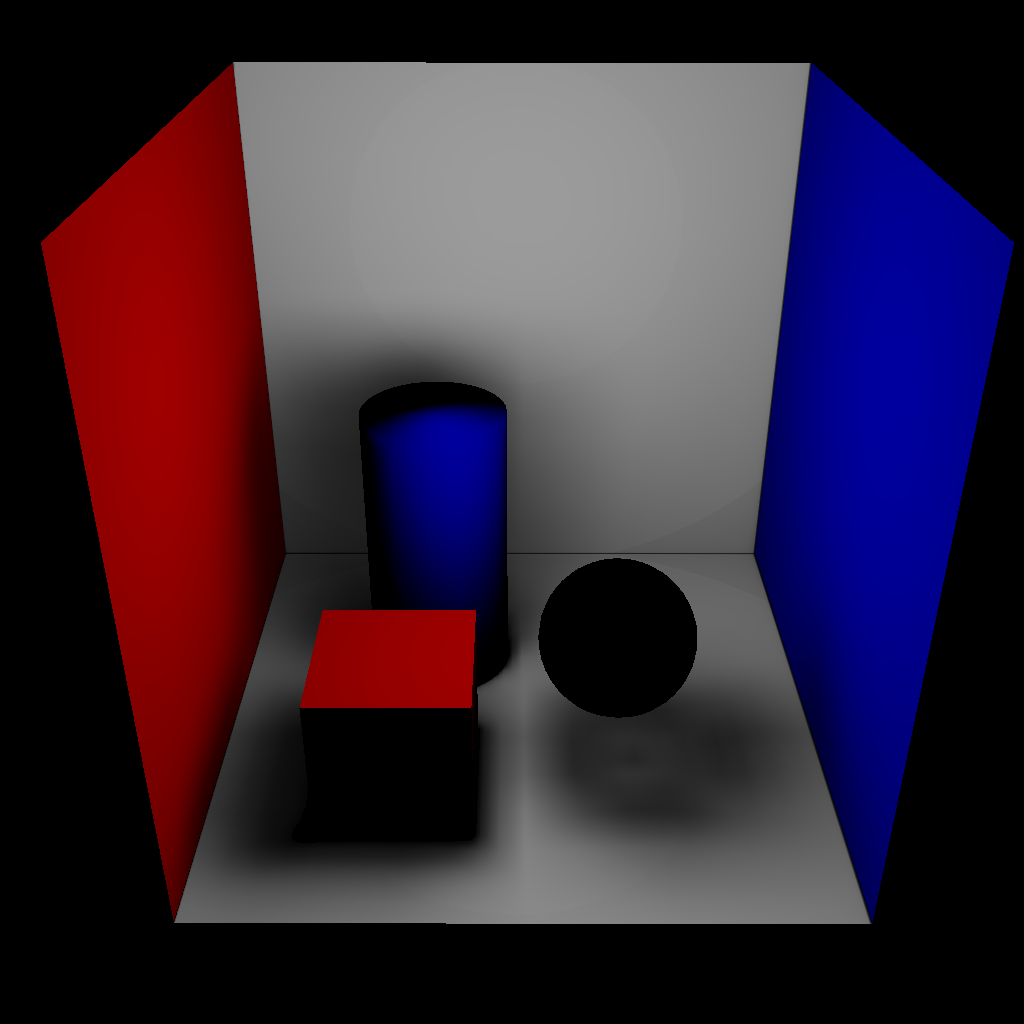
\includegraphics[width=\textwidth]{cornell-box-direct.png}
	      \caption{Solo luz directa.}
	  \end{subfigure}
	  \begin{subfigure}{0.49\textwidth}
	      \centering
	  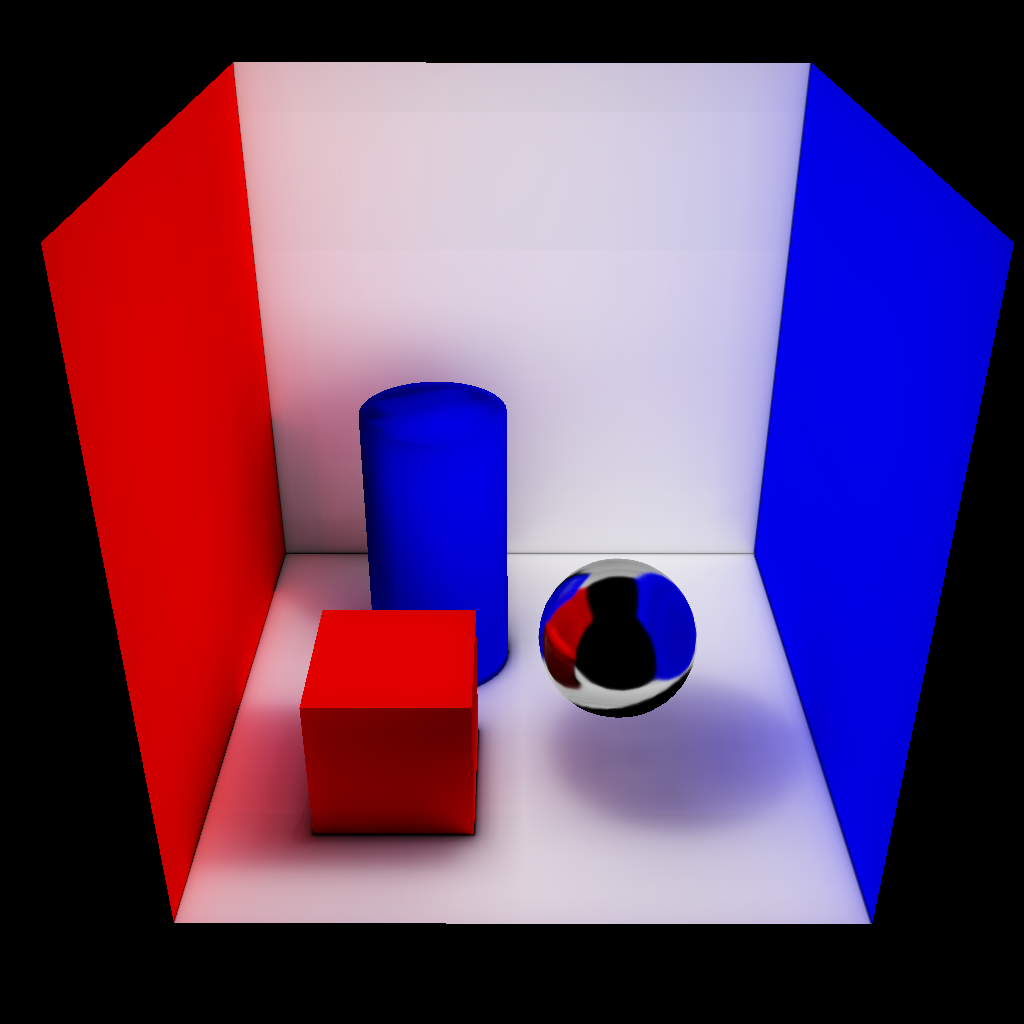
\includegraphics[width=\textwidth]{cornell-box-full.png}
	      \caption{Luz directa e indirecta.}
	  \end{subfigure}
	\caption{Escena de prueba con geometría simple.}
	\label{fig:cornell-box-full}
\end{figure}

\begin{figure}[H]
	\begin{subfigure}{0.49\textwidth}
	  \centering
	  \includegraphics[width=\textwidth]{sponza-direct.png}
	  \caption{Solo luz directa.}
	\end{subfigure}
	\begin{subfigure}{0.49\textwidth}
	  \centering
	  \includegraphics[width=\textwidth]{sponza-all.png}
	  \caption{Luz directa e indirecta.}
	\end{subfigure}
	\caption{Sponza.}
	\label{fig:sponza}
\end{figure}

Los experimentos varían la cantidad de vóxeles por dimensión, y registran los cuadros por segundo alcanzados (FPS, por sus siglas en inglés) y el tiempo de construcción del \textit{octree} en segundos.
Para conseguir los FPS se ejecutó el programa durante un minuto, tomando una muestra cada segundo, luego se promediaron.
Para el tiempo de construcción del \textit{octree}, se construyó 50 veces y se calculó el tiempo promedio.
Cada ejecución se realizó independientemente, para evitar posibles mejoras debido al uso del caché.

En el Cuadro \ref{tab:experiment-results} se muestran los resultados de estos experimentos en los 3 hardwares utilizados ($H1$, $H2$ y $H3$) descritos en el Cuadro \ref{tab:hardware-used}.
Se muestran los resultados para cada una de las escenas $S1$ y $S2$, en cada uno de los hardwares, y para cada nivel de resolución (vóxeles por dimensión).

\begin{table}[ht]
\centering
\begin{tabular}{|c|c|c|c|c|}
	\hline
	\textbf{Escena} & \textbf{Hardware} & \textbf{Vóxeles} & \textbf{FPS} & \textbf{Construcción del \textit{octree} (s)} \\
	\hline
	$S1$ & $H1$ & $256$ & $18.22$ & $1.76$ \\
	\cline{3-5}
	 & & $512$ & $14.77$ & $1.82$ \\
	\cline{3-5}
	 & & $1024$ & $12.13$ & $2.01$ \\
	\cline{2-5}
	 & $H2$ & $256$ & $136.57$ & $1.78$ \\
	\cline{3-5}
	 & & $512$ & $108.67$ & $1.80$ \\
	\cline{3-5}
	 & & $1024$ & $60.24$ & $1.89$ \\
	\cline{2-5}
	 & $H3$ & $256$ & $141.57$ & $1.88$ \\
	\cline{3-5}
	 & & $512$ & $141.47$ & $1.90$ \\
	\cline{3-5}
	 & & $1024$ & $140.88$ & $1.89$ \\
	\hline
	$S2$ & $H1$ & $256$ & $7.30$ & $1.84$ \\
	\cline{3-5}
	 & & $512$ & $4.29$ & $1.86$ \\
	\cline{3-5}
	 & & $1024$ & $2.84$ & $2.07$ \\
	\cline{2-5}
	 & $H2$ & $256$ & $59.68$ & $1.82$ \\
	\cline{3-5}
	 & & $512$ & $37.42$ & $1.94$ \\
	\cline{3-5}
	 & & $1024$ & $9.83$ & $1.83$ \\
	\cline{2-5}
	 & $H3$ & $256$ & $141.27$ & $1.70$ \\
	\cline{3-5}
	 & & $512$ & $141.51$ & $1.91$ \\
	\cline{3-5}
	 & & $1024$ & $141.21$ & $1.99$ \\
	\hline
\end{tabular}
\caption{FPS y tiempo de construcción del octree para cada escena.}
\label{tab:experiment-results}
\end{table}

\section{Análisis de resultados}

Una primera observación es que los cuadros por segundo se encuentran cerca del tiempo real.
Se nota que en $H1$ los FPS nunca superan los 20, mientras que en $H3$ nunca bajan de 140.
$H2$ representa un término medio, logrando más de 60 FPS en la escena simple ($S1$) y mostrando una gran variedad de valores en la escena compleja ($S2$) para cada resolución utilizada ($256$, $512$, $1024$).

Se observa que, como es de esperarse, a mayor resolución (vóxeles por dimensión), los cuadros por segundo disminuyen.
Esto se debe a que una resolución más alta mejora la aproximación y genera imágenes de mayor calidad, pero a costa de mayor carga computacional.

Un aspecto que destaca especialmente es el tiempo de construcción del octree, que permanece alrededor de los 2 segundos, cuando idealmente debería estar en el rango de los milisegundos.
Dado que este tiempo es prácticamente igual tanto en $H1$ como en $H3$, parece evidente que el cuello de botella no es la GPU en sí, sino la comunicación entre GPU y CPU.


% experimentación
\graphicspath{{chapters/5_experimentos/figures/}}

\chapter{Experimentación}\label{chap:experiments}

Para analizar el rendimiento de la implementación, se realizaron experimentos en distintas tarjetas gráficas, las cuales se ven en el Cuadro \ref{tab:hardware-used}.
Estas, $H1$, $H2$ y $H3$, corresponden a hardware con capacidades gráficas progresivamente superiores.
Las escenas utilizadas se muestran en las figuras \ref{fig:cornell-box-full} y \ref{fig:sponza}, que llamaremos $S1$ y $S2$ respectivamente.
Se puede observar en cada una de ellas la luz indirecta difusa, luz indirecta especular y sombras suaves.

\begin{table}[ht]
	\centering
	\begin{tabular}{|c|c|c|c|c|}
		\hline
		\textbf{Nombre} & \textbf{GPU} & \textbf{Núcleos} & \textbf{Clock (GHz)} & \textbf{VRAM (GB)} \\
		\hline
		$H1$ & Intel Mesa ADL GT2 & 96 & 1.45 & * \\
		\hline
		$H2$ & Nvidia GTX 1660 Ti mobile & 1536 & 1.45 & 6 \\
		\hline
		$H3$ & Nvidia Geforce RTX 4070 & 5888 & 1.92 & 12 \\
		\hline
	\end{tabular}
	\caption{Hardware utilizado. * al ser una tarjeta integrada, no tiene memoria gráfica dedicada.}
	\label{tab:hardware-used}
\end{table}

\begin{figure}[H]
	\centering
	  \begin{subfigure}{0.49\textwidth}
	      \centering
	  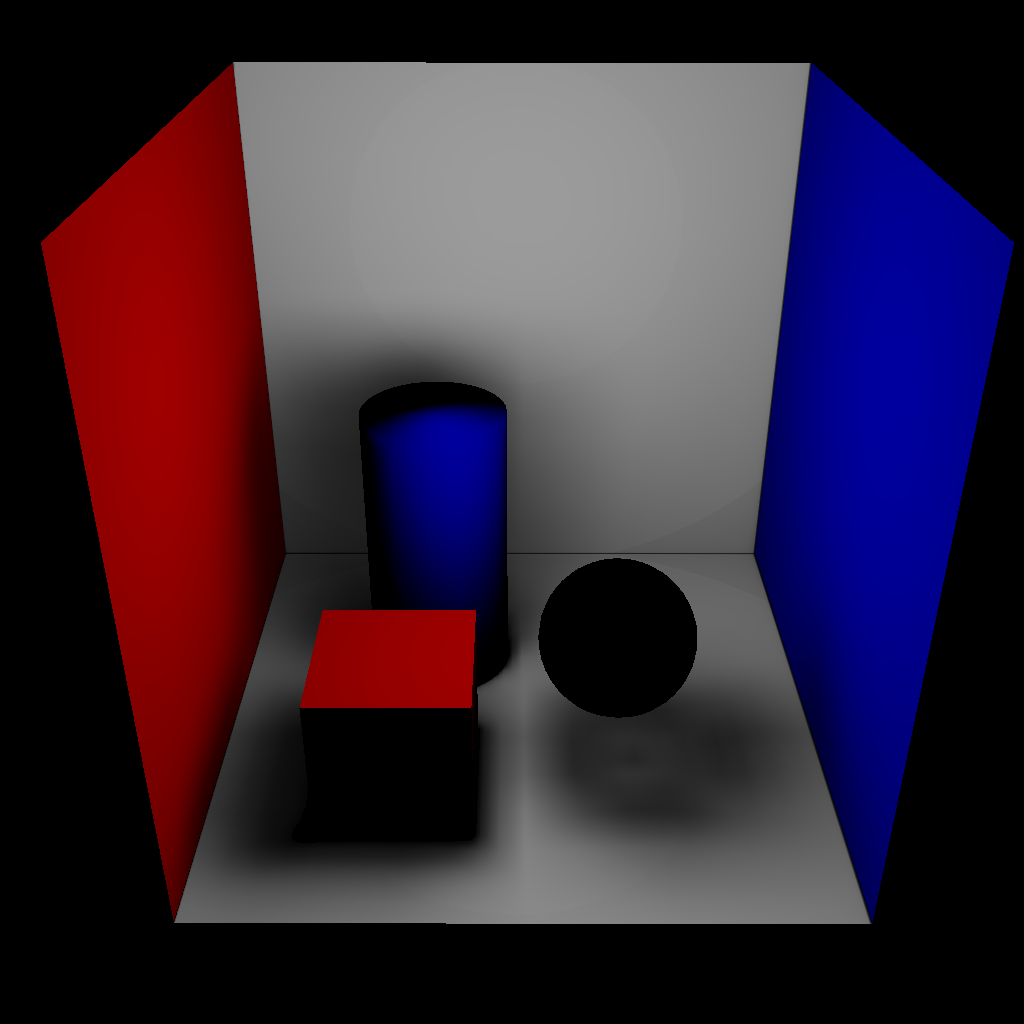
\includegraphics[width=\textwidth]{cornell-box-direct.png}
	      \caption{Solo luz directa.}
	  \end{subfigure}
	  \begin{subfigure}{0.49\textwidth}
	      \centering
	  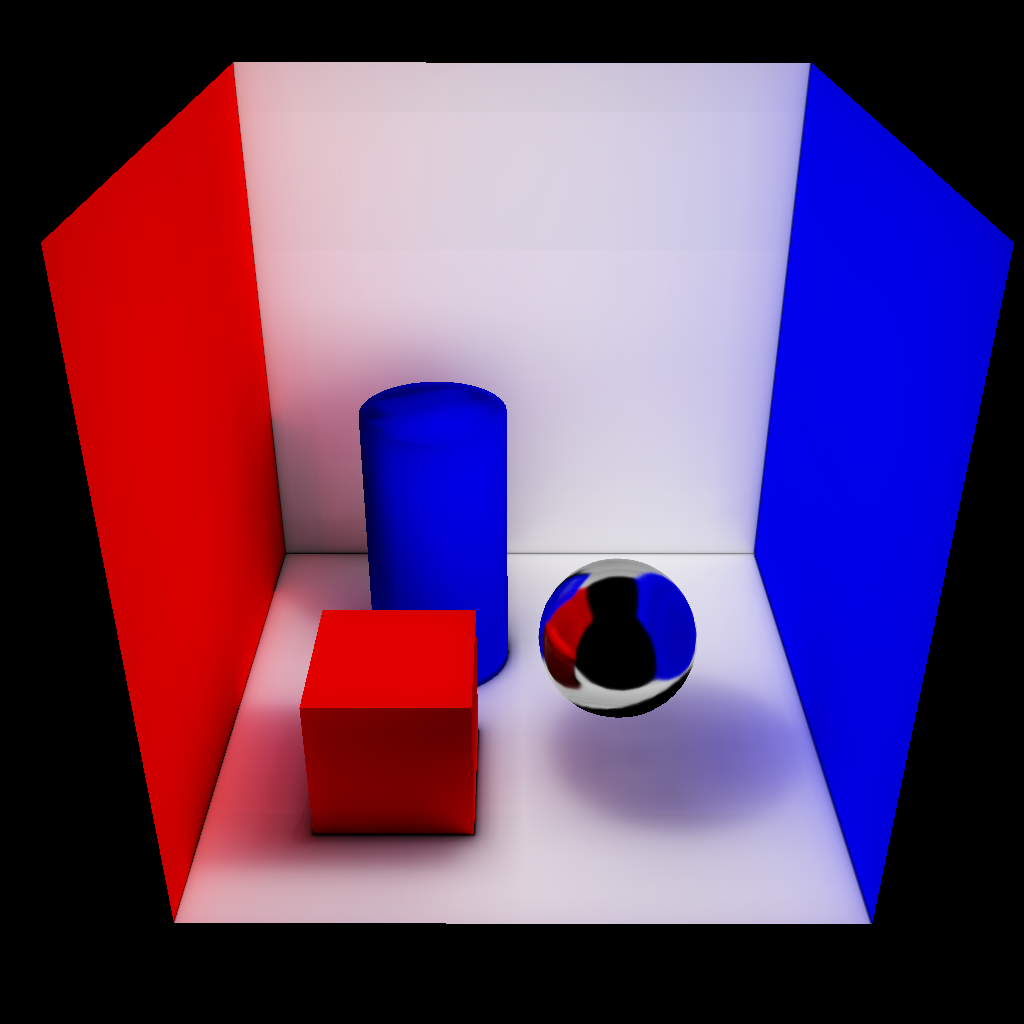
\includegraphics[width=\textwidth]{cornell-box-full.png}
	      \caption{Luz directa e indirecta.}
	  \end{subfigure}
	\caption{Escena de prueba con geometría simple.}
	\label{fig:cornell-box-full}
\end{figure}

\begin{figure}[H]
	\begin{subfigure}{0.49\textwidth}
	  \centering
	  \includegraphics[width=\textwidth]{sponza-direct.png}
	  \caption{Solo luz directa.}
	\end{subfigure}
	\begin{subfigure}{0.49\textwidth}
	  \centering
	  \includegraphics[width=\textwidth]{sponza-all.png}
	  \caption{Luz directa e indirecta.}
	\end{subfigure}
	\caption{Sponza.}
	\label{fig:sponza}
\end{figure}

Los experimentos varían la cantidad de vóxeles por dimensión, y registran los cuadros por segundo alcanzados (FPS, por sus siglas en inglés) y el tiempo de construcción del \textit{octree} en segundos.
Para conseguir los FPS se ejecutó el programa durante un minuto, tomando una muestra cada segundo, luego se promediaron.
Para el tiempo de construcción del \textit{octree}, se construyó 50 veces y se calculó el tiempo promedio.
Cada ejecución se realizó independientemente, para evitar posibles mejoras debido al uso del caché.

En el Cuadro \ref{tab:experiment-results} se muestran los resultados de estos experimentos en los 3 hardwares utilizados ($H1$, $H2$ y $H3$) descritos en el Cuadro \ref{tab:hardware-used}.
Se muestran los resultados para cada una de las escenas $S1$ y $S2$, en cada uno de los hardwares, y para cada nivel de resolución (vóxeles por dimensión).

\begin{table}[ht]
\centering
\begin{tabular}{|c|c|c|c|c|}
	\hline
	\textbf{Escena} & \textbf{Hardware} & \textbf{Vóxeles} & \textbf{FPS} & \textbf{Construcción del \textit{octree} (s)} \\
	\hline
	$S1$ & $H1$ & $256$ & $18.22$ & $1.76$ \\
	\cline{3-5}
	 & & $512$ & $14.77$ & $1.82$ \\
	\cline{3-5}
	 & & $1024$ & $12.13$ & $2.01$ \\
	\cline{2-5}
	 & $H2$ & $256$ & $136.57$ & $1.78$ \\
	\cline{3-5}
	 & & $512$ & $108.67$ & $1.80$ \\
	\cline{3-5}
	 & & $1024$ & $60.24$ & $1.89$ \\
	\cline{2-5}
	 & $H3$ & $256$ & $141.57$ & $1.88$ \\
	\cline{3-5}
	 & & $512$ & $141.47$ & $1.90$ \\
	\cline{3-5}
	 & & $1024$ & $140.88$ & $1.89$ \\
	\hline
	$S2$ & $H1$ & $256$ & $7.30$ & $1.84$ \\
	\cline{3-5}
	 & & $512$ & $4.29$ & $1.86$ \\
	\cline{3-5}
	 & & $1024$ & $2.84$ & $2.07$ \\
	\cline{2-5}
	 & $H2$ & $256$ & $59.68$ & $1.82$ \\
	\cline{3-5}
	 & & $512$ & $37.42$ & $1.94$ \\
	\cline{3-5}
	 & & $1024$ & $9.83$ & $1.83$ \\
	\cline{2-5}
	 & $H3$ & $256$ & $141.27$ & $1.70$ \\
	\cline{3-5}
	 & & $512$ & $141.51$ & $1.91$ \\
	\cline{3-5}
	 & & $1024$ & $141.21$ & $1.99$ \\
	\hline
\end{tabular}
\caption{FPS y tiempo de construcción del octree para cada escena.}
\label{tab:experiment-results}
\end{table}

\section{Análisis de resultados}

Una primera observación es que los cuadros por segundo se encuentran cerca del tiempo real.
Se nota que en $H1$ los FPS nunca superan los 20, mientras que en $H3$ nunca bajan de 140.
$H2$ representa un término medio, logrando más de 60 FPS en la escena simple ($S1$) y mostrando una gran variedad de valores en la escena compleja ($S2$) para cada resolución utilizada ($256$, $512$, $1024$).

Se observa que, como es de esperarse, a mayor resolución (vóxeles por dimensión), los cuadros por segundo disminuyen.
Esto se debe a que una resolución más alta mejora la aproximación y genera imágenes de mayor calidad, pero a costa de mayor carga computacional.

Un aspecto que destaca especialmente es el tiempo de construcción del octree, que permanece alrededor de los 2 segundos, cuando idealmente debería estar en el rango de los milisegundos.
Dado que este tiempo es prácticamente igual tanto en $H1$ como en $H3$, parece evidente que el cuello de botella no es la GPU en sí, sino la comunicación entre GPU y CPU.


%conclusiones
\graphicspath{{chapters/5_experimentos/figures/}}

\chapter{Experimentación}\label{chap:experiments}

Para analizar el rendimiento de la implementación, se realizaron experimentos en distintas tarjetas gráficas, las cuales se ven en el Cuadro \ref{tab:hardware-used}.
Estas, $H1$, $H2$ y $H3$, corresponden a hardware con capacidades gráficas progresivamente superiores.
Las escenas utilizadas se muestran en las figuras \ref{fig:cornell-box-full} y \ref{fig:sponza}, que llamaremos $S1$ y $S2$ respectivamente.
Se puede observar en cada una de ellas la luz indirecta difusa, luz indirecta especular y sombras suaves.

\begin{table}[ht]
	\centering
	\begin{tabular}{|c|c|c|c|c|}
		\hline
		\textbf{Nombre} & \textbf{GPU} & \textbf{Núcleos} & \textbf{Clock (GHz)} & \textbf{VRAM (GB)} \\
		\hline
		$H1$ & Intel Mesa ADL GT2 & 96 & 1.45 & * \\
		\hline
		$H2$ & Nvidia GTX 1660 Ti mobile & 1536 & 1.45 & 6 \\
		\hline
		$H3$ & Nvidia Geforce RTX 4070 & 5888 & 1.92 & 12 \\
		\hline
	\end{tabular}
	\caption{Hardware utilizado. * al ser una tarjeta integrada, no tiene memoria gráfica dedicada.}
	\label{tab:hardware-used}
\end{table}

\begin{figure}[H]
	\centering
	  \begin{subfigure}{0.49\textwidth}
	      \centering
	  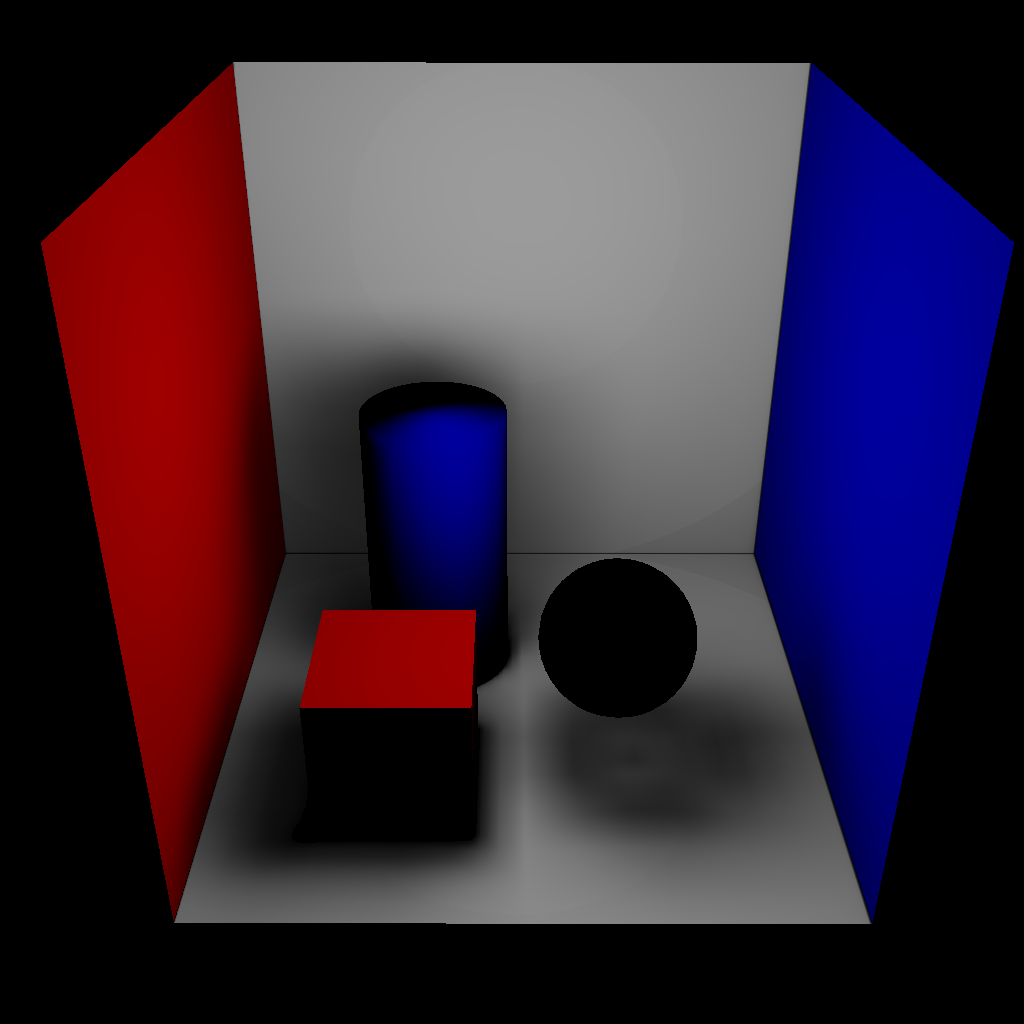
\includegraphics[width=\textwidth]{cornell-box-direct.png}
	      \caption{Solo luz directa.}
	  \end{subfigure}
	  \begin{subfigure}{0.49\textwidth}
	      \centering
	  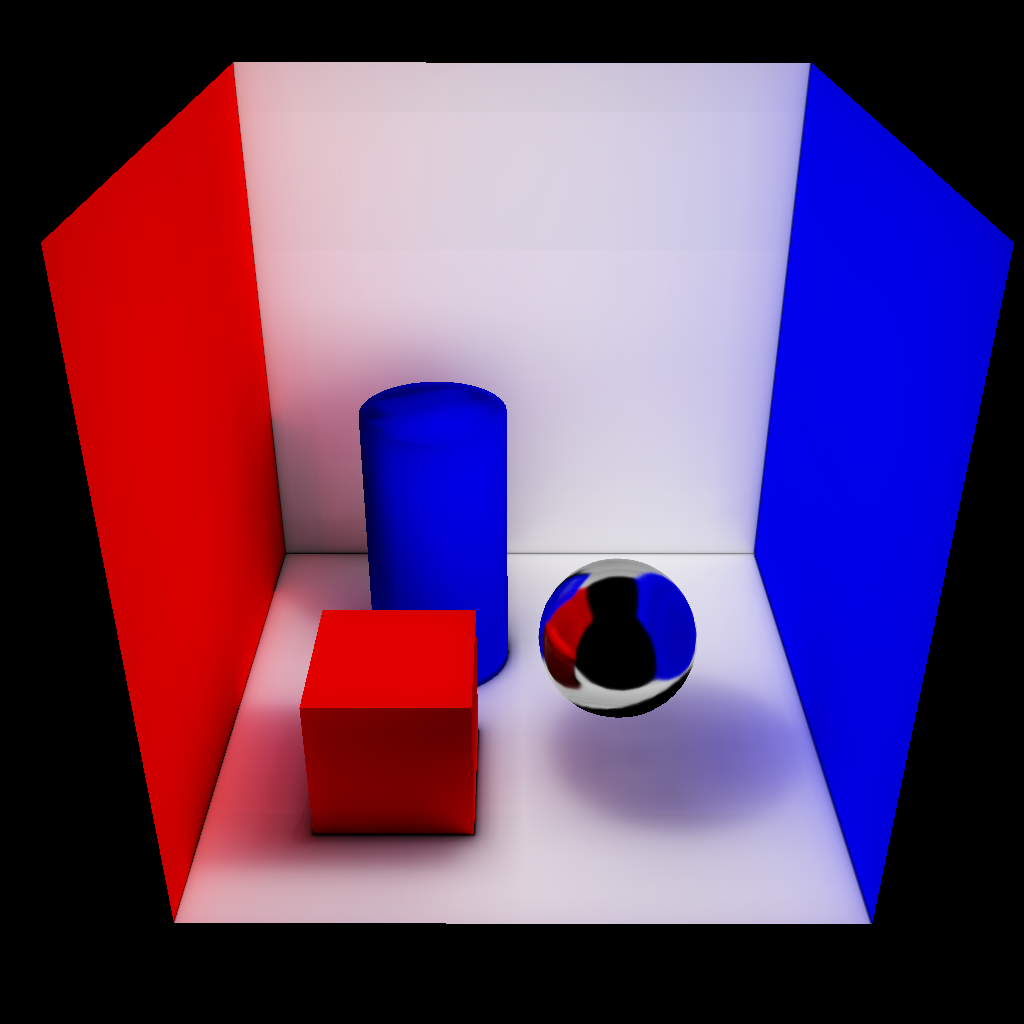
\includegraphics[width=\textwidth]{cornell-box-full.png}
	      \caption{Luz directa e indirecta.}
	  \end{subfigure}
	\caption{Escena de prueba con geometría simple.}
	\label{fig:cornell-box-full}
\end{figure}

\begin{figure}[H]
	\begin{subfigure}{0.49\textwidth}
	  \centering
	  \includegraphics[width=\textwidth]{sponza-direct.png}
	  \caption{Solo luz directa.}
	\end{subfigure}
	\begin{subfigure}{0.49\textwidth}
	  \centering
	  \includegraphics[width=\textwidth]{sponza-all.png}
	  \caption{Luz directa e indirecta.}
	\end{subfigure}
	\caption{Sponza.}
	\label{fig:sponza}
\end{figure}

Los experimentos varían la cantidad de vóxeles por dimensión, y registran los cuadros por segundo alcanzados (FPS, por sus siglas en inglés) y el tiempo de construcción del \textit{octree} en segundos.
Para conseguir los FPS se ejecutó el programa durante un minuto, tomando una muestra cada segundo, luego se promediaron.
Para el tiempo de construcción del \textit{octree}, se construyó 50 veces y se calculó el tiempo promedio.
Cada ejecución se realizó independientemente, para evitar posibles mejoras debido al uso del caché.

En el Cuadro \ref{tab:experiment-results} se muestran los resultados de estos experimentos en los 3 hardwares utilizados ($H1$, $H2$ y $H3$) descritos en el Cuadro \ref{tab:hardware-used}.
Se muestran los resultados para cada una de las escenas $S1$ y $S2$, en cada uno de los hardwares, y para cada nivel de resolución (vóxeles por dimensión).

\begin{table}[ht]
\centering
\begin{tabular}{|c|c|c|c|c|}
	\hline
	\textbf{Escena} & \textbf{Hardware} & \textbf{Vóxeles} & \textbf{FPS} & \textbf{Construcción del \textit{octree} (s)} \\
	\hline
	$S1$ & $H1$ & $256$ & $18.22$ & $1.76$ \\
	\cline{3-5}
	 & & $512$ & $14.77$ & $1.82$ \\
	\cline{3-5}
	 & & $1024$ & $12.13$ & $2.01$ \\
	\cline{2-5}
	 & $H2$ & $256$ & $136.57$ & $1.78$ \\
	\cline{3-5}
	 & & $512$ & $108.67$ & $1.80$ \\
	\cline{3-5}
	 & & $1024$ & $60.24$ & $1.89$ \\
	\cline{2-5}
	 & $H3$ & $256$ & $141.57$ & $1.88$ \\
	\cline{3-5}
	 & & $512$ & $141.47$ & $1.90$ \\
	\cline{3-5}
	 & & $1024$ & $140.88$ & $1.89$ \\
	\hline
	$S2$ & $H1$ & $256$ & $7.30$ & $1.84$ \\
	\cline{3-5}
	 & & $512$ & $4.29$ & $1.86$ \\
	\cline{3-5}
	 & & $1024$ & $2.84$ & $2.07$ \\
	\cline{2-5}
	 & $H2$ & $256$ & $59.68$ & $1.82$ \\
	\cline{3-5}
	 & & $512$ & $37.42$ & $1.94$ \\
	\cline{3-5}
	 & & $1024$ & $9.83$ & $1.83$ \\
	\cline{2-5}
	 & $H3$ & $256$ & $141.27$ & $1.70$ \\
	\cline{3-5}
	 & & $512$ & $141.51$ & $1.91$ \\
	\cline{3-5}
	 & & $1024$ & $141.21$ & $1.99$ \\
	\hline
\end{tabular}
\caption{FPS y tiempo de construcción del octree para cada escena.}
\label{tab:experiment-results}
\end{table}

\section{Análisis de resultados}

Una primera observación es que los cuadros por segundo se encuentran cerca del tiempo real.
Se nota que en $H1$ los FPS nunca superan los 20, mientras que en $H3$ nunca bajan de 140.
$H2$ representa un término medio, logrando más de 60 FPS en la escena simple ($S1$) y mostrando una gran variedad de valores en la escena compleja ($S2$) para cada resolución utilizada ($256$, $512$, $1024$).

Se observa que, como es de esperarse, a mayor resolución (vóxeles por dimensión), los cuadros por segundo disminuyen.
Esto se debe a que una resolución más alta mejora la aproximación y genera imágenes de mayor calidad, pero a costa de mayor carga computacional.

Un aspecto que destaca especialmente es el tiempo de construcción del octree, que permanece alrededor de los 2 segundos, cuando idealmente debería estar en el rango de los milisegundos.
Dado que este tiempo es prácticamente igual tanto en $H1$ como en $H3$, parece evidente que el cuello de botella no es la GPU en sí, sino la comunicación entre GPU y CPU.


\backmatter % no numerar capítulos 

% referencias bibliográficas

\newpage

\printbibliography

%%%%%%%%%%%%%%%%%%%%%%%%%%%%%%%%%%%%%%%%%%%%%%%%%%%%%%%%%%%%%%%%%%%%%%%%%%%%%%%%%%%%%%%%%%%%%%%%

% anexos

\begin{appendix}

% Manual de usuario
\graphicspath{{appendices/figures}}

\chapter{Anexo: Manual de Usuario}\label{appendix:manual}

En este anexo se presenta el manual de usuario del programa disponible en el siguiente repositorio de GitHub: \href{https://github.com/franciscoaguirre/voxel-cone-tracing}{https://github.com/franciscoaguirre/voxel-cone-tracing}.

El repositorio incluye un ejecutable localizado en la carpeta \textit{bin}, bajo el nombre \textit{cli}. Cabe destacar que dicho ejecutable es compatible únicamente con sistemas operativos Linux. En caso de emplear un sistema operativo diferente, será necesario compilar el ejecutable a partir del código fuente proporcionado.

\subsection{Compilación del Código Fuente}

Para compilar el código fuente, es indispensable tener instalado \href{Rust}{https://rustup.rs/}. Una vez instalado, la compilación se realiza mediante la ejecución del siguiente comando:

\texttt{cargo build --release}

\section{Opciones de Ejecución}

Si se ejecuta el programa sin especificar ninguna opción, este finalizará inmediatamente. Es necesario indicar qué escena se desea utilizar. En la carpeta \textit{scenes} se encuentran varios archivos de escena con la extensión \textit{.ron}. Para ejecutar una escena específica, debe añadirse la opción \texttt{--scene <nombre-escena>} al comando de ejecución, donde ``<nombre-escena>'' corresponde al nombre del archivo de la escena, sin incluir la extensión. Por ejemplo:

\texttt{./cli --scene cornell-box}

Además, el programa utiliza configuraciones definidas en el archivo \textit{config.ron}, donde se pueden ajustar parámetros como la resolución de la ventana y la resolución de la grilla de vóxeles.

El repositorio también incluye archivos de \textit{presets}, los cuales proporcionan un estado inicial para las escenas. Aunque se proporcionan algunos ejemplos generados automáticamente, más adelante se detallará cómo generar nuevos.

\section{Controles del Programa}

Una vez dentro del programa, con una escena cargada y sin un \textit{preset} activado, se pueden utilizar las teclas \textit{W}, \textit{A}, \textit{S}, \textit{D} o las flechas del teclado para mover la cámara. A continuación, se describen algunas de las funcionalidades clave:

\begin{itemize}
    \item Tecla \textit{1}: Muestra la escena cargada.
    \item Tecla \textit{2}: Muestra la versión voxelizada de la escena.
    \item Tecla \textit{C}: Permite mover la fuente de luz, representada por un cubo blanco vacío. Los efectos de la luz se visualizarán cuando se activen opciones de iluminación directa o indirecta desde el menú.
\end{itemize}

\subsection{Acceso al Menú}

El menú principal se accede mediante la tecla \textit{Escape}, y proporciona acceso a varios submenús para el control detallado de diferentes aspectos del programa.

\begin{figure}[h]
    \centering
    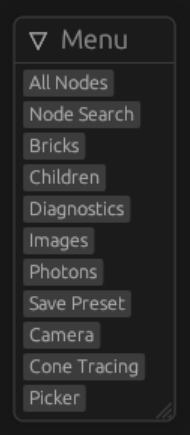
\includegraphics[width=.5\textwidth]{menu.png}
    \caption{Menú Principal.}
    \label{fig:menu}
\end{figure}

Como se observa en la figura \ref{fig:menu}, los submenús disponibles son:

\begin{itemize}
	\item All Nodes
	\item Node Search
	\item Bricks
	\item Children
	\item Diagnostics
	\item Images
	\item Photons
	\item Save Preset
	\item Camera
	\item Cone Tracing
	\item Picker
\end{itemize}

A continuación, se describen en detalle cada uno de estos.

\subsubsection{All Nodes}

Este submenú permite visualizar la representación gráfica del \textit{octree} y ajustar el nivel de detalle mostrado. En la figura \ref{fig:all_nodes} se muestra el botón que activa la visualización del \textit{octree} y el \textit{slider} que permite controlar los niveles.

\begin{figure}[h]
    \centering
    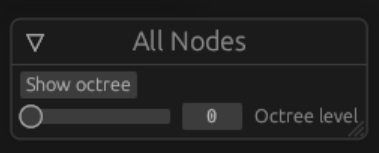
\includegraphics[width=.5\textwidth]{all_nodes.png}
    \caption{Submenú \textit{All Nodes}.}
    \label{fig:all_nodes}
\end{figure}

\subsubsection{Node Search}

Este submenú ofrece la funcionalidad de buscar nodos del \textit{octree} ya sea por índice o posición. Al seleccionar un nodo de la lista, este se muestra en el espacio de la escena. Además, existe la opción de destacar los nodos vecinos al nodo seleccionado, y es posible seleccionar múltiples nodos. Este menú ha sido de gran utilidad durante el proceso de depuración del programa. La figura \ref{fig:node_search} ilustra su uso.

\begin{figure}[h]
    \centering
    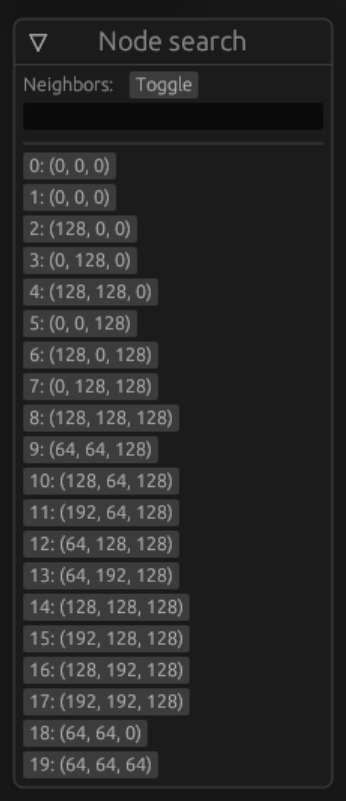
\includegraphics[width=.5\textwidth]{node_search.png}
    \caption{Submenú \textit{Node Search}.}
    \label{fig:node_search}
\end{figure}

\subsubsection{Bricks}

Este submenú, a diferencia de los anteriores que muestran nodos, permite visualizar los bricks asociados a esos nodos. La figura \ref{fig:bricks} muestra las distintas opciones disponibles. Para limitar el impacto en el rendimiento, es posible visualizar una capa de vóxeles de los bricks a la vez. Asimismo, se pueden visualizar el color y la irradiancia de los vóxeles, así como las normales de los mismos.

Los controles situados al final del submenú permiten cambiar la dirección desde la cual se observan los bricks, algo relevante dado que los vóxeles son filtrados anisotrópicamente.

\begin{figure}[h]
    \centering
    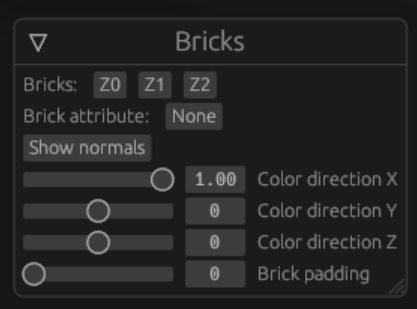
\includegraphics[width=.5\textwidth]{bricks.png}
    \caption{Submenú \textit{Bricks}.}
    \label{fig:bricks}
\end{figure}

\subsubsection{Children}

Al seleccionar un nodo utilizando el submenú \textit{Node Search}, este submenú muestra los atributos del nodo seleccionado. La figura \ref{fig:children} muestra este submenú con y sin un nodo seleccionado. Una vez seleccionado un nodo $n$, se presentan los índices de sus nodos hijos, los cuales pueden ser posteriormente buscados en el submenú \textit{Node Search}.

\begin{figure}[h]
    \begin{center}
    \begin{subfigure}{.49\textwidth}
        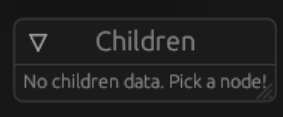
\includegraphics[width=\textwidth]{children-off.png}
        \caption{Sin nodo seleccionado.}
    \end{subfigure}
    \begin{subfigure}{.49\textwidth}
        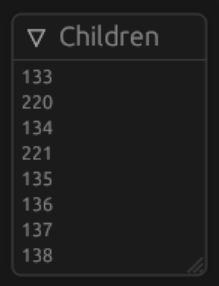
\includegraphics[width=\textwidth]{children-on.png}
        \caption{Con nodo seleccionado.}
    \end{subfigure}
    \caption{Submenú \textit{Children}.}
    \label{fig:children}
    \end{center}
\end{figure}

\subsubsection{Diagnostics}

El submenú \textit{Diagnostics} proporciona información sobre el rendimiento de la aplicación, específicamente los cuadros por segundo (FPS), como se muestra en la figura \ref{fig:diagnostics}.

\begin{figure}[h]
    \centering
    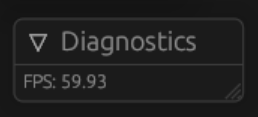
\includegraphics[width=.5\textwidth]{diagnostics.png}
    \caption{Submenú \textit{Diagnostics}.}
    \label{fig:diagnostics}
\end{figure}

\subsubsection{Images}

Este submenú permite mostrar diferentes imágenes en pantalla, de manera similar a cómo las teclas \textit{1} y \textit{2} permiten mostrar la escena original y la versión voxelizada respectivamente. En la figura \ref{fig:images}, se presentan las opciones disponibles:

\begin{itemize}
    \item Color: Muestra la escena original, equivalente a presionar la tecla \textit{1}.
    \item Direct Light: Muestra la escena iluminada únicamente por la luz directa.
    \item Indirect Diffuse: Muestra la escena iluminada por la luz indirecta difusa reflejada en las superficies.
    \item Indirect Specular: Muestra la escena iluminada por la luz indirecta especular reflejada en superficies brillantes o metálicas.
    \item Ambient Occlusion: Muestra la escena en escala de grises de acuerdo con la oclusión ambiental en cada punto.
\end{itemize}

Cada una de estas opciones añade un efecto adicional a la imagen, permitiendo una visualización progresiva de los diferentes elementos de la iluminación.

\begin{figure}[h]
    \centering
    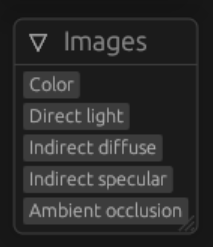
\includegraphics[width=.5\textwidth]{images.png}
    \caption{Submenú \textit{Images}.}
    \label{fig:images}
\end{figure}

\subsubsection{Photons}

Este submenú, similar al submenú \textit{Children}, muestra la cantidad de fotones en cada vóxel del brick de un nodo seleccionado previamente en el submenú \textit{Node Search}.

\subsubsection{Save Preset}

Este submenú permite guardar todas las configuraciones seleccionadas en el menú en un archivo de \textit{preset}.
Para guardar, simplemente se debe elegir un nombre para el archivo y presionar el botón \textit{Save}, como se muestra en la figura \ref{fig:save_preset}.
Estos archivos pueden ser cargados en futuras ejecuciones utilizando la opción \texttt{--preset <nombre-archivo>}.

\begin{figure}[h]
    \centering
    
\includegraphics[width=.5\textwidth]{save_preset.png}
    \caption{Submenú \textit{Save Preset}.}
    \label{fig:save_preset}
\end{figure}

\subsubsection{Camera}

Este submenú permite cambiar la proyección de la cámara a una vista ortogonal.

\subsubsection{Cone Tracing}

Este submenú ofrece control sobre la apertura y la distancia máxima de los conos utilizados para sombras, oclusión ambiental, reflexión difusa, reflexión especular y conos de prueba. La figura \ref{fig:cone_tracing} ilustra estas opciones.

\begin{figure}[h]
    \centering
    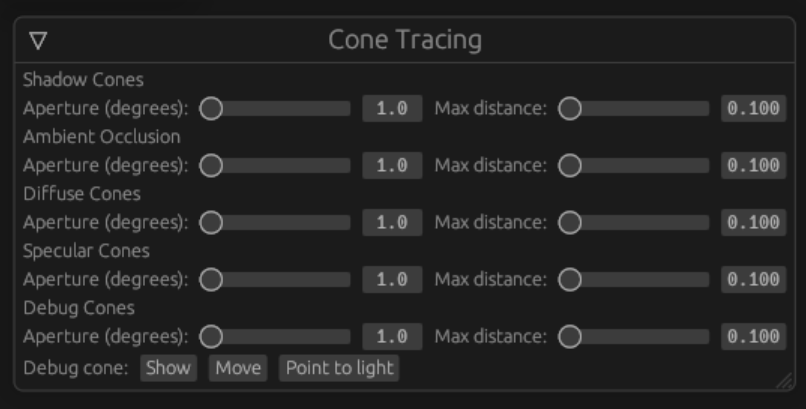
\includegraphics[width=.5\textwidth]{cone_tracing.png}
    \caption{Submenú \textit{Cone Tracing}.}
    \label{fig:cone_tracing}
\end{figure}

\subsubsection{Picker}

Este submenú permite activar un modo en el cual el cursor puede ser utilizado para seleccionar un punto en la pantalla y lanzar un cono desde ese punto en la escena. El submenú se muestra en la figura \ref{fig:picker-menu}, y un ejemplo del cono de prueba en acción se presenta en la figura \ref{fig:picker-action}. El cono de prueba muestra los nodos a través de los cuales pasa.

\begin{figure}[h]
    \centering
    \includegraphics[width=.5\textwidth]{picker-menu.png}
    \caption{Submenú \textit{Picker}.}
    \label{fig:picker-menu}
\end{figure}

\begin{figure}[h]
    \centering
    \includegraphics[width=.5\textwidth]{picker-action.png}
    \caption{Cono de prueba en acción.}
    \label{fig:picker-action}
\end{figure}


\end{appendix}

%%%%%%%%%%%%%%%%%%%%%%%%%%%%%%%%%%%%%%%%%%%%%%%%%%%%%%%%%%%%%%%%%%%%%%%%%%%%%%%%%%%%%%%%%%%%%%%%

\end{document}
